% Tento soubor nahraďte vlastním souborem s obsahem práce.
%=========================================================================
% Autoři: Michal Bidlo, Bohuslav Křena, Jaroslav Dytrych, Petr Veigend a Adam Herout 2019

% Pro kompilaci po částech (viz projekt.tex), nutno odkomentovat a upravit
%\documentclass[../projekt.tex]{subfiles}
%\begin{document}
\chapter{Úvod}
\label{chapter:1}
Dnes, v~21. století, máme na výběr tolik informací, jako jsme ještě nikdy neměli. Poprvé jsme nuceni vybírat si informace a kontrolovat, zda jsou pravdivé a objektivní nebo naopak lživé a zavádějící. Jak víme, že to, co nám média prezentují, je objektivní? Není možné, že nám ukazují jen část pravdy, tu část, kterou chtějí?

Především v~televizních a rozhlasových médiích jsou populární relace (v~zahraničí přezdívané Q\&A), ve kterých se diváci dotazují moderátora, známých osobností či odborníků na různé otázky, které chtějí zodpovědět. Jsme schopni zjistit, zda otázky, které jsou položeny skrze různé aplikace, byly nějak zmanipulovány nebo cenzurovány? Jednotlivé dotazy tak mohly být neoprávněně pozměněny, skryty či odstraněny. Spolu s~tím je možné, že všechny otázky byly položeny pouze produkčním týmem nebo jednotlivci, kteří se pod rouškou internetu vydávají za \uv{běžné} publikum.
% zodpovědět
Smyslem této práce je vytvořit koncept decentralizované mobilní aplikace, ve které bude uživatel pokládat jednotlivé otázky. Aplikace přinese přínos v~tom, že díky použití technologie zvané blockchain nedovolí žádné straně cenzurovat ani manipulovat otázky. Druhou, neméně cennou předností bude, že uživatelé, kteří se budou chtít zúčastnit relace, si musí ověřit svoji identitu. To zamezí umělému navyšování počtu otázek a zajistí tak přirozený průběh relace. Využití aplikace by mohlo nastat především ve veřejnoprávních médiích, která by měla být objektivní a transparentní, ale i kdekoliv na internetu. \\
% cenzurovat otázky ani s nimi manipulovat
\section{Struktura práce }
V~kapitole \ref{chapter:2} jsou vysvětleny potřebné pojmy spojené s~blockchainem, které jsou nutné k~pochopení problematiky. Kapitola \ref{chapter:3} stručně popisuje programovací prostředí pro vývoj mobilních aplikací. Dále ve \ref{chapter:4}. kapitole si představíme použité technologie potřebné k~vytvoření práce. \ref{chapter:5}. kapitola vysvětluje přínos práce a porovnává již existující aplikace. V~kapitole \ref{chapter:6} si popíšeme použité smart kontrakty a aplikace. Nakonec v~\ref{chapter:7}. kapitole dojde na otestování aplikace a samotné zhodnocení práce. 
% na otestování aplikace a NA samotné?
% doplnit podle zpětné vazby bezpečnost/diskuzi?
\chapter{Potřebné znalosti k~pochopení decentralizovaných aplikací}
\label{chapter:2}
Přestože je tu blockchain již déle než 10 let, nacházejí se mezi informatiky tací, kteří o~něm moc nevědí. Pro vytvoření decentralizované aplikace je nutné si vysvětlit základní pojmy, které nám pomohou chápat problematiku blockchainu a decentralizovaných aplikací. V~případě, že se kdekoliv v~této práci budeme bavit o~adrese nebo transakci, budou vždy tyto pojmy znamenat blockchainovou adresu a blockchainovou transakci.

Na následujících stránkách si proto vysvětlíme pojmy jako blockchain, konsenzus, smart kontrakt nebo decentralizovaná aplikace a pojmy s~nimi spojené.

\section{Blockchain a jeho části}
Historie blockchainu sahá až do roku 2008, kdy neznámý autor (případně skupina autorů) pod pseudonymem Satoshi Nakamoto sepsal první návrh fungování blockchainu, ze kterého vyšla první kryptoměna zvaná Bitcoin \cite{Nakamoto2008}. Koncept blockchainu a Bitcoinu byl reakcí na~nedostatky tradičního bankovního systému. Pro potřeby této práce definujeme blockchain jako distribuovanou decentralizovanou databázi, která ukládá veškeré informace o~transakcích, které proběhly mezi uživateli systému \cite{Bashir2017}. Na obrázku \ref{fig:topologie} jsou znázorněny rozdílné síťové topologie. Mezi nesporné výhody decentralizovaného blockchainu patří neschopnost data smazat nebo je jakkoli upravit. Díky tomu se objem dat postupem času může pouze navyšovat.
% TODO_HM 
% Na obrázku 2.1 jsou zobrazeny rozdílné síťové topologie, ze kterých blockchain vychází?/které blockchain používá? Které pomohou pochopit blockchain?

\begin{figure}
\centering
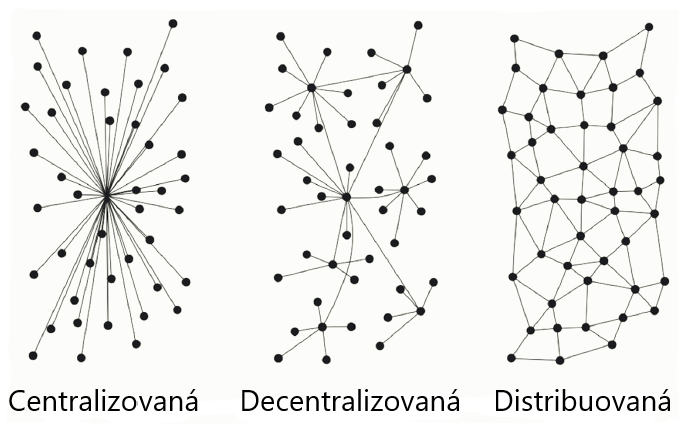
\includegraphics[width=\textwidth]{obrazky/centralized-vs-decentralized-vs-distributed-processing.png}
\caption{Typy síťových topologií \cite{Topologie}} 
\label{fig:topologie}
\centering
\end{figure}

\subsection*{Základní stavební kámen blockchainu: Blok a jeho vlastnosti}
V~terminologii blockchainu si pod pojmem blok představme datovou strukturu. Dělí se na 2 hlavní části, hlavičku a tělo \cite{blok}. Mezi součásti hlavičky patří hash hlavičky předchozího bloku, Merkle root (hash všech transakcí zahrnutých v~bloku, česky kořenový uzel), časové razítko a hodnota nonce. V~těle se nachází seznam transakcí včetně jejich dat. Části bloku jsou znázorněny na obrázku \ref{fig:blok}. Hash hlavičky nám udává jednoznačný identifikátor bloku, který se uloží do následujícího bloku. Tímto způsobem se bloky utvářejí v~jeden dlouhý řetězec (blockchain). Časové razítko symbolizuje čas zařazení bloku do řetězce. Nonce je číslo, které se přidává k~datům v~bloku a slouží k~tomu, aby se vypočítal hash bloku  \cite{Bitcoin_block}. 

V~případě, že by v~bloku proběhla i byť nepatrná změna, narušila by celý řetězec, protože by došlo k~přepočítání hashe hlavičky. Tento mechanismus zajišťuje, že bloky v~blockchainu nelze jednoduše modifikovat bez povšimnutí, což zvyšuje důvěru a bezpečnost této technologie. Nutno ještě podotknout, že v~odlišných implementacích blockchainu se struktura bloku může lišit.

\begin{figure}
\centering
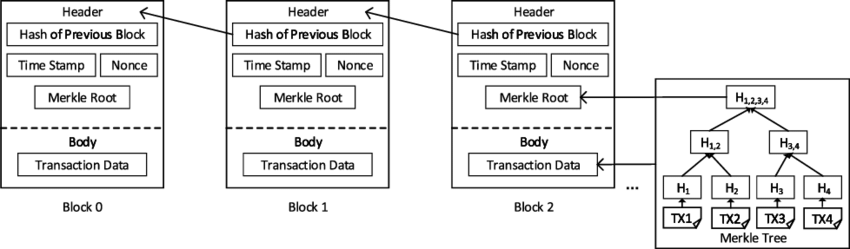
\includegraphics[width=\textwidth]{obrazky/block.png}
\caption{Schéma blockchainu \cite{Schema}}
\label{fig:blok}
\centering
\end{figure}

\subsection*{Transakce v~blockchainu}
Významem blockchainových transakcí je převod prostředků mezi adresami v~síti \cite{Bashir2017}. Nicméně to není jejich jedinou úlohou. V~závislosti na implementaci blockchainu mohou zajišťovat i uložení trvalých informací do blockchainu, protože odesílatel je schopen do nich vložit i určitý objem metadat. V~tomto ohledu se podobají tedy databázovým transakcím, které mění uložená data databáze. My se bavíme o~případě, kde databází je blockchain. 

Samotné transakce však nejsou uskutečněny okamžitě, nýbrž se nejprve slučují do tzv.~mempoolů. Každý těžař (pojem těžař bude vysvětlen dále) má vlastní mempool, ze kterého vybírá transakce do bloku a kde uspořádává transakce podle výše poplatku, který je v~konečném pojetí jeho odměnou. V~aktivních špičkách sítě je nutné zaplatit buď vyšší poplatek nebo počkat, až těžař vybere transakci a zařadí ji do bloku. Vše je samožřejmě podmíněno škálovatelností sítě a dalšími parametry, které ovlivňují množství a rychlost zpracovaných transakcí. Ve chvíli, kdy je transakce zapsána do bloku a tudíž se provedla, je nutné počkat na určitý počet potvrzení, tzn. kolik bloků bylo po zveřejnění transakce zapsáno do blockchainu (doporučený počet potvrzení bloku v~Ethereu je 12, což trvá zhruba 3~minuty). Tato vlastnost se nazývá finalita bloku. Dlouhý čas do finality bloku může přinést náhodné forky, které vytvářejí paralelní nekonzistentní zobrazení blockchainu \cite{transaction}. 

V~případě, že uživatel nepočká dostatečně dlouho, může se jeho transakce prohlásit za neplatnou. Na obrázku \ref{fig:retezec} vidíme černě nejdelší řetězec bloků a modře dočasné paralelní větvě, které se mohly jevit v~danou chvíli jako nejdelší. Mohlo by se totiž stát, že se najde jiný a delší řetězec bloků, který uznají uzly v~síti jako hlavní, v~němž by se daná transakce nemusela nacházet a tudíž by byla neplatná \cite{Transaction_confirmations}. Existují ale blockchainy, jejichž finalita bloků je velice rychlá a zmíněné problémy zde nenastávají.  
% může se jeho transakce - se může jeho transakce
\subsection*{Uzel v~blockchainové síti}
Uzel (angl. node) se primárně podílí na konsenzu blockchainu (viz sekce \ref{konsenzus}) a sekundárně slouží jako uložiště informací blockchainu. V~uzlech jsou uloženy částečné nebo celé řetězce bloků (kopie blockchainu). Mohli bychom je přirovnat k~serverům, které taktéž ukládají potřebné informace pro uživatele. Mezi jejich další činnost lze zařadit legitimaci bloků s~transakcemi či zasílání nových dat pomocí broadcastu ostatním uzlům \cite{Abrol2022}. 

Není ale uzel jako uzel a proto je dobré poznamenat, v~čem se odlišují. Opět jsou rozdílné podle implementace blockchainu a dělí se na 2 základní typy - full node a light node. Full node je uzel, který v~sobě uchovává celou kopii blockchainu a je zpravidla odpovědný za ověřování transakcí a bloků v~blockchainové síti. Jeho podtypem je konsenzuální uzel (angl. konsenzus node), který odpovídá za těžbu nových bloků a jejich přidávání do blockchainu. Light node v~sobě uchovává pouze část blockchainu a zpravidla se jedná o~hlavičky bloků~\cite{Node2018}.

\begin{figure}
\centering
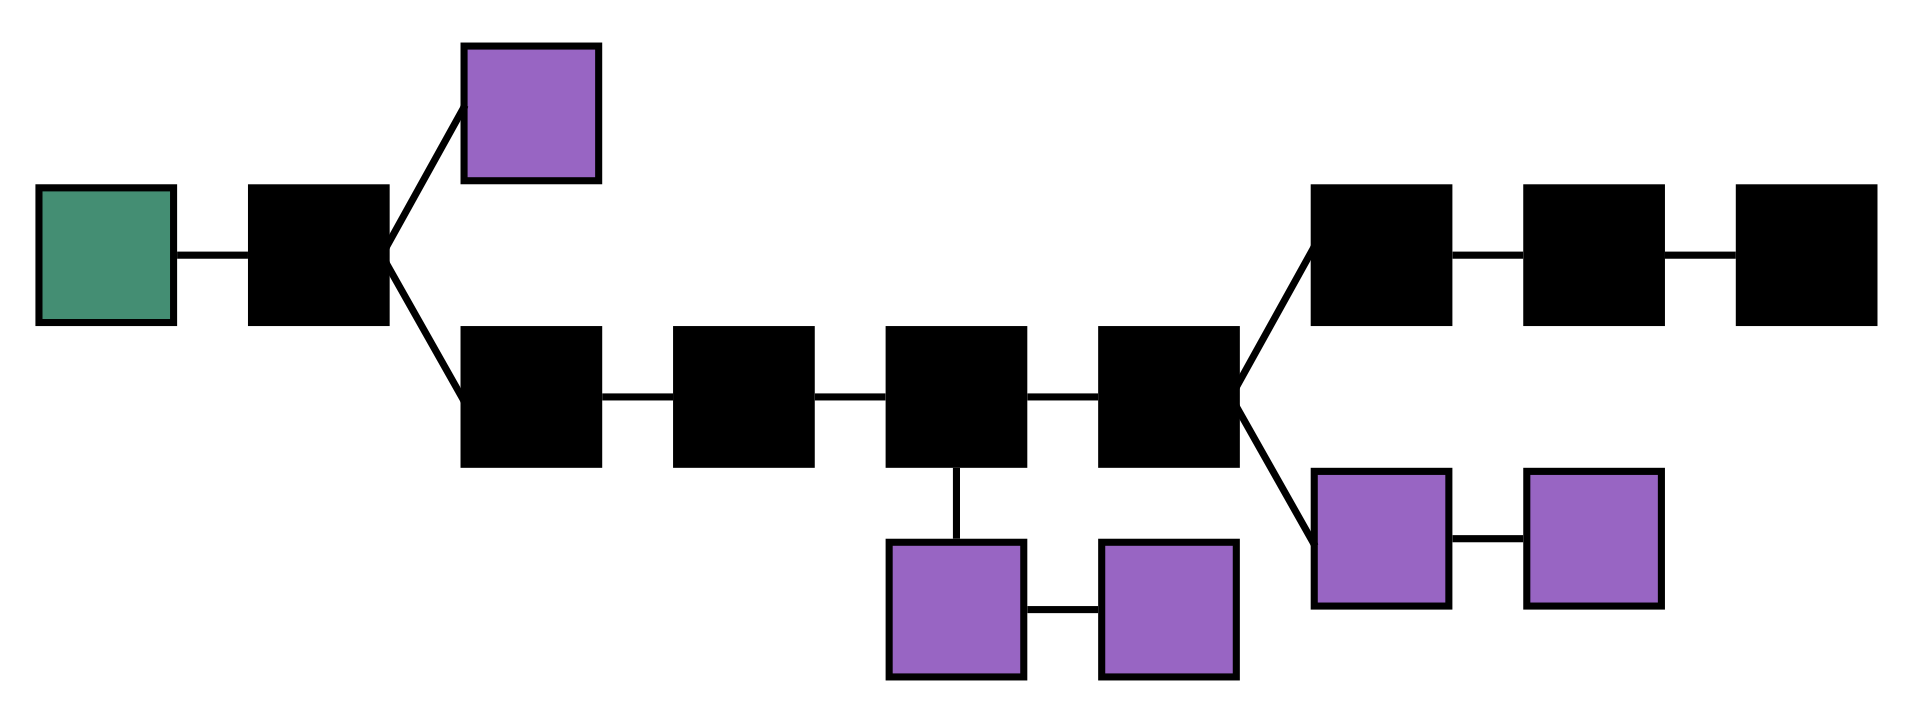
\includegraphics[width=\textwidth]{obrazky/vetve_bloku.png}
\caption{Řetězec schválených bloků \cite{longestChain}}
\label{fig:retezec}
\centering
\end{figure}

\section{Konsenzus v~blockchainu: Zajištění konzistence a integrity sítě} 
\label{konsenzus}
K~čemu je dobré se v~blockchainu shodnout? Abychom zajistili jediný zdroj pravdy v~celé blockchainové síti a aby všechny uzly měly dostupné stejné a pravdivé informace. Výstupem této shody je blok, který bude zařazen do blockchainu. Tento proces se nazývá konsenzus. Díky němu se uživatelé sítě blockchainu dohodnou na tom, jaký blok vybrat i přes to, že si vzájemně nedůvěřují \cite{Lashkar2021}. Za tímto procesem stojí konsenzuální uzly, které za vidinou odměny v~podobě nativní kryptoměny a poplatků přidávají do dané sítě bloky. Aby vůbec mohli bloky přiřadit do blockchainu, musí vložit určitou hodnotu jako zálohu, nejčastěji se jedná o~výpočetní sílu nebo nativní měnu sítě. Tato záloha by měla odradit uzly od nečestného chování, jelikož by jim při jejich prohřešku nebyla vrácena. Konsenzuální uzly a způsoby, jak konsenzu dosáhnout, se napříč blockchainovými sítěmi liší. Následující podkapitoly obsahují nejznámější typy konsenzuálních protokolů dohody \cite{Binance}.
% mohli?
%hodnotu jako zálohu? - hodnotu
\subsection*{Proof of work}
Anglicky proof of work (zkr. PoW), česky důkaz práce je první a nejstarší z~možností, jak dojít ke konsenzu v~blockchainové síti. Způsobem, kterým docílit shody mezi všemi uzly v~síti je obětování značného množství výpočetní síly k~vyřešení \uv{kryptografického puzzle} \cite{POW}. Těžař (angl. miner), jakožto osoba (případně skupina osob), která se snaží toto puzzle řešit, musí najít na základě konkrétních vstupů předem definovaný hash při minimální odchylce. Svoji odpověď následně odešle do sítě, kde poté ostatní uživatelé snadno ověří řešení a pokud je opravdu správné, nálezce získá odměnu. Složitost této činnosti závisí na celkové výpočetní síle všech těžařů, tzv. hashrate \cite{POW_POS}. Při použití PoW je vysoká spotřeba elektrické energie, zacož je tento algoritmus mnohdy kritizován. Jeho hlavním konkurentem je Proof of Stake (zkr. PoS), který byl kvůli negativní spotřebě energie PoW algoritmu vytvořen. 
% česky důlaz práce - do závorky, případně za čárku?
% za což?
\subsection*{Proof of stake}
Principem proof of stake (česky důkaz podílu) je ověřování blokových transakcí na základě počtu \uv{investovaných} mincí \cite{POS}. Tento mechanismus motivuje uživatele k~držení a použití mincí jako zástavy (tzv. stake) za vidinou zisku transakčních poplatků. Jednotliví validátoři (uživatelé, kteří mají zastavené mince) jsou vybírání náhodně, kde pravděpodobnost jejich zvolení je přímo úměrná počtu vsazených mincí. Bloky jsou validovány více validátory a po ověření správnosti bloku je samotný blok finalizován a uzavřen \cite{POW_POS}. Jednotlivé blockchainové sítě mohou mít různě implementovaný PoS, který se pro běžné uživatele liší primárně v~minimálním možném počtu mincí, které musí být zastaveny, aby mohli obdržet odměnu za validaci transakcí. Např. u~sítě Ethereum je minimální vsazené množství 32 ETH \cite{ETH}, což aktuálně (21.3.2023) činí zhruba 1,25 milionu Kč \cite{coinmarketcap}. Samotný PoS by měl snížit oproti PoW riziko centralizace a nabízet validátorům lepší vstupní podmínky, nicméně nedosažitelné vstupy k~decentralizaci nepřispívají. Pro mnohé uživatele není možné investovat takový obnos peněz a proto byly vytvořeny tzv. staking pooly, do kterých uživatelé delegují jen určitou část potřebnou pro stake \cite{ethereum}. Odměna je následně počítána podle množství investovaných prostředků. V~PoW je také typické se sdružovat, a to do tzv. mining poolů.
% k datu (21.3.2023) ?
\section{Definice a vlastnosti smart kontraktů v~blockchainu}
\label{section:sc}
Prvotní myšlenka implementace smart kontraktů, (angl. smart contract) vznikla v~roce 1994 ústy Nicka Szaba. Tou bylo provádět automatizované procesy bez nutnosti důvěry ve třetí stranu \cite{eth_sc}. \uv{Je zaručeno, že smart kontrakty budou probíhat předem definovaným a deterministickým způsobem, bez zásahů žádné konkrétní třetí strany} \cite{Voshmgir2017}. Samotnou definici můžeme tedy popsat následovně: Smart kontrakt je kód nasazený v~prostředí blockchainu, který je vyvolán blockchainovou transakcí při splnění určitých podmínek a způsobuje změnu stavu blockchainu nebo čte jeho hodnoty \cite{SC}. Při vytváření smart kontraktu bychom měli dbát na jeho maximální optimalizaci, protože každá instrukce stojí určitý poplatek v~síti, tzv. gas. Uveďme si několik výhod, které smart kontrakty skýtají:

\begin{itemize}
    \item Vyšší efektivitu kontraktů, a to pomocí kontroly kontraktu uživateli, který je kdykoliv dostupný a zároveň nemožnosti zanést do nich chyby prostřednictvím jejich ručního přepisování.
    \item Odstranění nutné důvěry mezi smluvními stranami, jelikož je kontrakt proveden na základě předem stanovených podmínek bez potřeby prostředníka, s~čímž se pojí i nižší náklady. I~přesto je někdy nutné pomocí centralizovaného prostředníka dodat data do blockchainu.
    \item Nezávislost na centrální autoritě.
\end{itemize}
% vyšší efektivita?
Bohužel lze najít i několik nevýhod, se kterými musíme počítat:

\begin{itemize}
    \item Nutné zabezpečení kódu a ověření jeho správnosti. 
    \item Nevratnost kontraktů. V~případě, že nastane v~kódu chyba nebo jiný omyl, nelze se vrátit do stavu před jeho vykonáním.
    \item Oproti běžným smlouvám nelze smart kontrakty soudně vymáhat. 
    \item Nemožnost úpravy tradičního smart kontraktu po jeho nasazení. To však neplatí v~rámci \uv{upgradeable contracts}, které lze upravit i beze změny jejich adresy \cite{upgradable}. Je proto nutné, aby se změnou souhlasily pomocí hlasování všechny zúčastněné strany a nedošlo tak k~nečestnému jednání.
\end{itemize}
%upgradeable - uvozovky?
% souhlasily
Někomu nevýhody mohou připadat jako zanedbatelné, avšak opak je pravdou. V~případě širší adopce je nezbytné všechny nedokonalosti smart kontraktů důkladně zvážit a být velice obezřetný, protože by mohly nadělat více trápení než užitku. Většina implementací smart kontraktů v~právní oblasti stále ještě není zdaleka přijata nebo dokonce není nijak užitečná. Jedním z~důvodů, kromě toho, že je to poměrně pořád nové téma, je způsob přenosu citlivých a relevantních informací do smart kontraktů. Proto se občas musíme spolehnout na takzvané \uv{oracles} - služby důvěryhodných třetích stran, jejichž prostřednictvím jsou příslušné vstupy do kontraktů poskytovány. Blockchain sám o~sobě neumí používat jiná data, než jaká jsou v~něm uložená \cite{fintech}.
% zdaleka - ani zdaleka?
% oracles - uvozovky
\subsection*{Ethereum Virtual Machine: principy a architektura}
Jedná se o~nejznámější a nejrozšířenější platformu pro nasazení smart kontraktů. Ethereum Virtual Machine (zkr. EVM) je stavový stroj, který „zpracovává výpočty a stavy kontraktů a je postaven na zásobníkovém jazyce s~předdefinovanou sadou instrukcí a odpovídajících argumentů“ \cite{WohrerZdun}. Dílčí smart kontrakty se však nepodobají strukturou nízkoúrovňovým programovacím jazykům, které používají jednoduché sady instrukcí, ale naopak vysokoúrovňovým jazykům používající vlastnosti jako polymorfismus nebo dědičnost. Tento kód se až při překladu právě pomocí EVM překládá na jednoduché instrukce. Namísto specifických programovacích jazyků by bylo možné psát kód v~instrukcích, avšak by to bylo zbytečně složité. 

Jak je popsáno v~předchozí kapitole, jednotlivé instrukce mají svou cenu a stojí určitý poplatek. Cena některých instrukcí je znázorněna v~obrázku \ref{fig:instrukce}. Účelem těchto poplatků bylo, aby autoři byli nuceni psát optimální kódy a zamezilo se tak zbytečně dlouhým kódům, díky kterým by se mohl virtuální stroj přetížit \cite{WohrerZdun}. Můžeme říci, že EVM je prostředím, ve kterém existují všechny účty a chytré smlouvy Etherea \cite{evm}. Tento virtuální stroj rozhodně není jediným napříč blockchainy. Mnoho dalších sítí má své stroje, jako například NEO, Cardano, EOS atd. Ovšem nezáleží jen na výběru platformy, ale i na jazyce smart kontraktů, který ovlivní samotný vývoj decentralizované aplikace. Podívejme se tedy, s~čím lze EVM využít. 

\begin{figure}
\centering
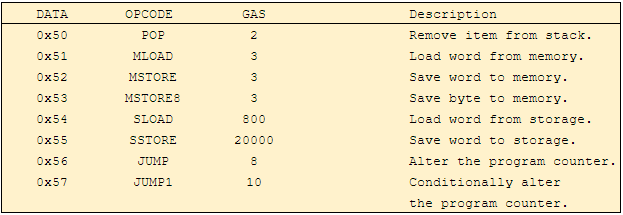
\includegraphics[width=\textwidth]{obrazky/instrukce.png}
\caption{Cena jednotlivých instrukcí \cite{yellowpaper}}
\label{fig:instrukce}
\centering
\end{figure}

\subsection*{Solidity}
Programovací jazyk Solidity slouží pro tvorbu smart kontraktů na platformě Ethereum \cite{solidity1}. V~blockchainové komunitě (a hlavně díky té okolo Etherea) patří mezi uživatelsky nejoblíbenější a nejrychleji rostoucí jazyky pro vytváření smart kontraktů. Jeho vývoj závisí na komunitě, která ho posouvá stále kupředu. Solidity je vysokoúrovňový staticky typovaný jazyk a jeho syntaxe se podobá stálicím jako C++, Python nebo JavaScript. Podobně i Solidity nabízí vlastnosti jako polymorfismus, dědičnost či použití externích knihoven. 
% díky té?
% vysokoúrovňový, doplnit čárku, staticky ...?
Dílčí smart kontrakty se podobají třídám u~objektově orientovaných jazyků a vyžadují přítomnost konstruktoru, který je vykonán při nasazení smlouvy do blockchainu. Jednotlivé části kódu je nutné zapisovat do funkcí, které jsou vyvolány uživateli sítě \cite{WohrerZdun}. Solidity nabízí použití speciálních proměnných v~globálním prostředí, které slouží k~poskytnutí informací o~blockchainu nebo samotných transakcích. Týká se to proměnných \texttt{block}, \texttt{msg} nebo \texttt{tx} \cite{eth_variables}. \texttt{Block} zahrnuje informace o~bloku, kupříkladu číslo aktuálního bloku či jeho časové razítko, \texttt{msg} poskytuje informace například o~odesílateli transakce či hodnotě wei, která je zaslána transakcí a \texttt{tx} zase třeba výši poplatku za transakci (gas). Další speciální vlastností Solidity je nativní funkce \texttt{require}, která slouží k~ověření podmínek ve funkcích. Pokud není podmínka splněna, funkce se ukončí s~chybovou hláškou nadefinovanou v~těle \texttt{require}. Na obrázku \ref{fig:solidity} je znázorněno použití speciální proměnné \texttt{msg} i funkce \texttt{require}. Dále nabízí i datovou strukturu \texttt{mapping}, která se velice podobá asociativnímu poli nebo slovníku u~jiných jazyků. 
% gas? -> tzv. gas
% Dále nabízí - Solidity dále nabízí?
\begin{figure}
\centering
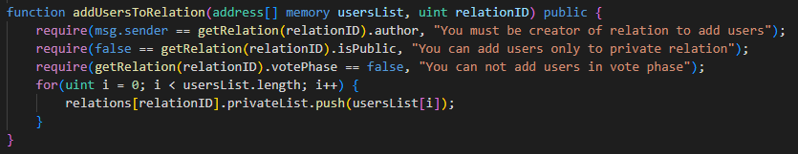
\includegraphics[width=\textwidth]{obrazky/Solidity.png}
\caption{Funkce \texttt{addUsersToRelation} z~vytvořeného smart kontraktu \texttt{Queans} sloužící k~přídaní uživatelů do soukromé relace, jazyk Solidity}
\label{fig:solidity}
\end{figure}

\subsection*{Vyper}
Obdobně jako Solidity je Vyper jazyk orientovaný na vytváření smart kontraktů, jejichž nasazení probíhá na EVM. Samotný Vyper je pythonský silně typovaný programovací jazyk, mezi jehož hlavní cíle se řadí následující vlastnosti \cite{vyper1}: 
\begin{itemize}
\item Bezpečnost -- Vyper by měl být schopen přirozeně produkovat bezpečné smart kontrakty.
\item Jednoduchost -- Implementace jazyka a kompilátoru by měly být jednoduché.
\item Auditovatelnost -- Kód psaný ve Vyperu má být pro člověka co nejčitelnější a zároveň musí být složité napsat zavádějící kód.
\end{itemize}

Vyper je natolik jednoduchým jazykem, že zde nenajdeme dědičnost, rekurzivní volání ani přetěžování operátorů či funkcí. Počet funkcí je záměrně omezen na co nejmenší počet, díky čemuž jsou kontrakty bezpečnější a snáze kontrolovatelné \cite{vyper2}. Samotný jazyk nevznikl jako konkurent Solidity, ale má ho doplňovat svou zvýšenou bezpečností \cite{vyper3}.
% TODO_HM 
% pythonský? - podobný pythonu? pythonický? 
% za python.. čárka?
% implementace by měly - měla?
\begin{figure}
\centering
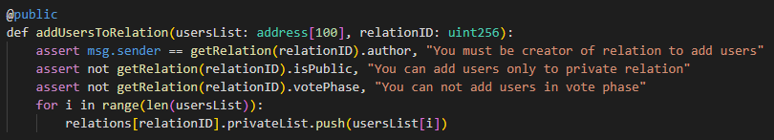
\includegraphics[width=\textwidth]{obrazky/Vyper.png}
\caption{Funkce z~obrázku \ref{fig:solidity} napsaná v~jazyce Vyper}
\end{figure}

\subsection*{Scilla}
Scilla je staticky typovaný jazyk pro tvorbu smart kontraktů. Obdobně jako Vyper se zaměřuje na jejich bezpečnost, zejména v~oblasti DeFi (decentralizované finance) \cite{scilla1}. Tento jazyk je vědecky ověřován a zvýšení bezpečnosti by měl zajistit skenr, který pomocí formální verifikace a statické analýzy dokáže hledat potenciální chyby, bezpečnostní problémy a další nedostatky v~kódu. Scilla byl navržen tak, aby byl jednoduchý na použití, ale zároveň dostatečně silný na to, aby umožnil programátorům psát komplexní smart kontrakty \cite{scilla2}.
% decentralizované finance
\begin{figure}
\centering
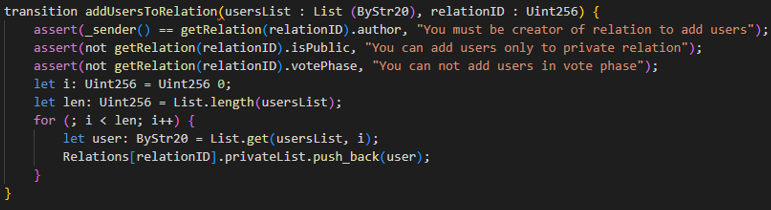
\includegraphics[width=\textwidth]{obrazky/Scilla.png}
\caption{Funkce z~obrázku \ref{fig:solidity} napsaná v~jazyce Scilla}
\centering
\end{figure}

\section{Decentralizované aplikace a jejich přínosy}
Decentralizované aplikace (zkr. dAPPs) jsou aplikacemi běžícími na blockchainu. Oproti centralizovaným aplikacím běží v~uživatelském prohlížeči a nejsou tudíž závislé na centralizovaném serveru, ze kterého fungují centralizované aplikace. Druhým rozdílem je, že využívají jako databázi blockchain, respektive stavy jednotlivých kontraktů a jejich proměnných. Fungují jako rozhraní, skrze které uživatel dokáže měnit stav sítě pomocí vyvolaných transakcí ze smart kontraktů, které má blockchain v~sobě uložen. Ideální blockchainová aplikace by měla být provozuschopná bez jakéhokoli lidského zásahu \cite{dapps}. Zde uvedu 4 body, které by měly ziskové dAPPs splňovat \cite{Raval2016}: 
% blockchain jako databázi
\begin{itemize}
\item Open source zdrojový kód -- Každá decentralizovaná aplikace by měla mít volně dostupný kód. Uživatelé, kteří chtějí využít jejích služeb by měli mít možnost si zkontrolovat zdrojový kód a sami vyhodnotit, zda nemá aplikace chyby nebo pochybná místa v~kódu. Open source kód může být ale dvousečnou zbraní a v~konkurenčním světě poskytne konkurenci velkolepý užitek.
\item Interní měna -- Jakým způsobem si vývojář dAPP vydělá peníze za provoz svojí aplikace? Jestliže jeho aplikace má open source kód a její provoz je zpoplatněn, může ji kdokoliv odcizit, mírně poupravit a nabídnout zdarma. Proto se vývojáři uchylují k~vytvoření interního tokenu (měny), jehož cena roste v~závislosti na použití aplikace. Následně pak svůj podíl tokenů mohou prodat a těšit se ze zisku.
\item Decentralizovaný koncenzus -- Je nespornou výhodou, kterou blockchain nabízí. Pro všechny aplikace, které vyžadují shodu všech uživatelů na určitých problémech, je blockchain správnou cestou. Nejedná se o~to, kdo kupříkladu finalizoval poslední blok v~síti, ale o~to, že se všichni shodnou na tom, že se to konkrétní osobě povedlo.
\item Žádný centrální bod selhání -- Blockchainová síť obsahuje nespočet nezávislých uzlů, které udržují síť při životě. V~případě, že některý z~nich selže, ostatní uzly to nijak neohrozí a jsou dále provozuschopné. Decentralizované aplikace tedy nelze jednoduše vypnout, protože jejich existence závisí na již zmíněných uzlech v~síti a ne na konkrétním centrálním serveru.
\end{itemize}

V~čem se decentralizovaná aplikace liší od té běžné centralizované? Proč by alespoň v~nějakých oblastech měly dAPPs převládat? Pokusím se nastínit konkrétní výhody a nevýhody, které mohou určit, zda by vývojář měl vůbec nad těmito možnostmi uvažovat a jestli mu mohou faktické rozdíly usnadnit nebo naopak zkomplikovat jeho práci \cite{dappProsCons}. \\
% běžné *čárka* centralizované?
Výhody dAPPs:

\begin{itemize}
\item Smart kontrakty by měly nabídnout ochranu soukromí uživatelů. Kontrakty spolu mohou komunikovat bez nutnosti napojení na centralizovanou stranu, která by byla schopna zneužít citlivá data uživatelů.
% by měly
\item Síť není závislá na centrálním serveru a tudíž stačí jediný dostupný uzel, aby nedošlo k~výpadku aplikace, přestože její výkon může být v~danou chvíli snížen.

\item Nepožadují vysoké náklady na instalaci serveru, včetně údržby a jeho správy a v~konečném důsledku jsou náklady na provoz minimální.

\item Neexistuje zde žádný centrální bod, který by mohl ohrozit bezpečnost aplikace. 

\item Decentralizované aplikace jsou odolné vůči cenzuře. Tato výhoda bude pro naši aplikaci zásadní.

\item Poskytují podnikatelskou příležitost pro nové uživatele. Neexistuje zde žádný subjekt, který by blokoval vstup na trh či jinak kontroloval uživatele.
 \end{itemize}

Nevýhody dAPPs:
\begin{itemize}
\item Nedostatečně prozkoumaná technologie, vývoj je v~počáteční fázi a netuší se, jak by aplikace fungovaly při jejich vysokém zatížení či zatížení sítě.
% fungovaly
\item Náročnost provádění úprav zdrojového kódu za účelem vylepšení nebo opravy chyb. Samotné aplikace se musí po úpravě znovu nasadit na blockchain. Výjimku tvoří dAPPs s~využitím \uv{upgradeable contracts}. Tento bod souvisí s~nevýhodami smart kontraktů ze sekce \ref{section:sc}.
% upgradeable - uvozovky?
\item Při špatně zvolené síti může nastat v~dAPP problém s~dlouhou dobou potvrzení transakce a tedy čekáním uživatelů na vykonání určité změny v~aplikaci.
%  tedy čekáním uživatelů
\item Přestože se snažíme vyhnout opakovanému zanesení chyb do smart kontraktů, jsme pouze lidé a je téměř jisté, že v~kódu budou chyby obsaženy.
% se snažíme se vyhnout?
\item Dříve či později se zveřejní aplikace, které nám svoji podstatou mohou škodit. Díky jejich decentralizaci je nebudeme schopni dobře omezit.
\end{itemize}

Jak jsme si zmínili, dAPPs mohou mít své plusy i mínusy. Jejich osvojení širokou veřejností však ještě chvíli potrvá. Nejdříve bude zapotřebí usnadnit vývojářům vývoj aplikací, ale i přiblížení nových možností běžným uživatelům. Někteří tvrdí, že tyto aplikace mohou být převratným bodem v~mnoha odvětvích. Ve finančním sektoru se jedná o~zlevnění transakčních poplatků, které aktuálně inkasují banky a velké finanční korporace, dále budou schopny zastoupit roli autoritativních společností, ukládat a dále používat bezpečně naše citlivá data či nahradit sociální média a umožnit všem vyjadřovat svobodně své názory \cite{DAPPS2}. Jednoduše řečeno, možností je nespočet. Pouze a jen čas nám ukáže, jakým směrem se budou decentralizované aplikace ubírat.

\chapter{Programovací prostředí pro vývoj mobilních aplikací}
\label{chapter:3}
V~této kapitole projdeme možnosti vývoje mobilních aplikací a jejich programovací prostředí. Nabízí se nám 3 základní varianty vývoje, jimiž jsou nativní, webové nebo multiplatformní \cite{mobiles}. Rozhodující faktor pro výběr, jakým způsobem aplikaci tvořit, není většinou jeden, ale je jich celá řada. Jedná se například o~celkové náklady na vývoj, kvalitu vzhledu aplikace, platformu pro cílové uživatelé nebo rychlost aplikace \cite{AppsFrameworks}. Dále je potřeba vzít na vědomí, zda máme i schopné vývojáře, kteří umí používat konkrétní programovací jazyk nebo framework a vyznají se v~problematice mobilních aplikací. Přeci jenom je to trochu něco jiného, než tvořit aplikaci pro počítač.

\section{Nativní aplikace}
V~první řadě se od webových a multiplatformních aplikací liší tím, že cílí pouze na jednu konkrétní platformu. Mezi nejznámější platformy patří Android a iOS, případně sem lze zařadit i  Windows či Blackberry. Rozhraní nativních aplikaci jsou vždy spojena s~mobilním operačním systémem a tyto aplikace tak mohou přistupovat ke všem nativním API, jako jsou Bluetooth, geolokace, mikrofon nebo kamera \cite{mobiles}. Výhodou nativního přístupu je velice přívětivé uživatelské rozhraní, dobrá výkonnost aplikací a poměrně příznivá škálovatelnost samotné aplikace, nicméně vyvíjení nativních aplikací se pojí s~vyšší časovou, ale i finanční náročností. Pro vývoj se používá jazyk konkrétní platformy, v~případě Androidu se jedná o~Javu nebo Kotlin a v~případě iOS o~jazyk Swift nebo Objective-C \cite{mobilesuptech}. Dnešním problémem je taktéž nedostatek zkušených programátorů nativních aplikací, kteří by měli vysokou zkušenost s~vývojem těchto specifických aplikací \cite{mobilesamazon}. Pro přesun aplikací na jinou platformu je nutné přepsat kód, jelikož nelze jednoduše pozměnit. To stejné platí pro změnu frontendu aplikace \cite{mobilesibm}. Má vůbec cenu vyvíjet nativním způsobem?
% TODO
% rozhraní jsou spojeny/spojena
\section{Multiplatformní aplikace}
Multiplatformní (hybridní) aplikace jsou kombinací nativních a webových aplikací. Jejich jedinečná vlastnost je, že jsou dostupné napříč všemi platformami s~použitím jediného kódu \cite{mobiles}. Občas se tento přístup nazývá \uv{write-once-run-anywhere} \cite{mobilesibm} .Výkonnost je oproti nativním aplikacím běžně nižší a to stejné platí i pro flexibilitu. Je mnohdy obtížné použít nativní funkce, jako fotoaparát, mikrofon nebo geolokaci. Zároveň s~tím jsou ale menší časové a finanční náklady, které jsou vykoupeny kvalitou výsledných aplikací. Multiplatformní aplikace se tvoří ve frameworcích jako React Native, Flutter či Xamarin \cite{mobilesuptech}.  Zatímco React Native poskytuje nativní komponenty pro práci s~multiplatformním kódem, Flutter a Xamarin kompilují tento kód do nativního kódu pro lepší výkon \cite{mobilesamazon}. 
% nativní funkce, jako??
%zároveň s tím - se s tím pojí?
\subsection*{Flutter}
Jedná se o~open-source framework pro tvorbu mobilních aplikací pro různé platformy vyvinutý společností Google v~roce 2017.  Jeho silné stránky jsou vykreslovací engine, testovací a integrační rozhraní API a widgety. Vykreslovací engine zodpovídá za rasterizaci scén při změně obrazu \cite{flutter}. Widgety slouží ve Flutteru jako \uv{stavební bloky} a každý objekt je widget. Tento framework nejenže nabízí širokou škálu předem vytvořených widgetů, ale také umožňuje uživatelům je tvořit a upravovat \cite{flutter2}. Flutter používá programovací jazyk Dart, který představuje klientsky optimalizovaný a staticky typovaný objektově orientovaný programovací jazyk. Dart je schopen kompilace do nativního kódu pro konkrétní mobilní zařízení. Samotný Flutter dokonce umožňuje rozšířit stávající mobilní projekt na web a počítač \cite{flutter3}. Kladem frameworku je i fakt, že nabízí funkci okamžitého načtení aplikace po její změně, kterou při vývoji ocení každý vývojář.
% staticky typovaný čárka ??
% na web a pc nebo pro web a pc?
\subsection*{React Native}
Jde opět o~open-source framework pro vývoj hybridních mobilních aplikací vytvořený organizací Meta (dříve Facebook) začátkem roku 2015 používající oblíbený jazyk JavaScript \cite{reactnative}. React Native je znám především svoji rozsáhlou komunitou, která se aktivně stará o~chod všech knihoven. Ty jsou nedílnou součástí frameworku React Native, protože nabízejí rychlý vývoj aplikací pro Android i iOS. Na základě toho můžeme říci, že je framework velmi kompatibilní s~pluginy třetích stran \cite{flutter2}. React Native vychází z~frameworku React používaného pro vývoj webových aplikací, ale umožňuje používat nativní prvky uživatelského rozhraní v~mobilních aplikacích. To je možné díky abstrakční vrstvě známé jako \uv{bridge}, která umožňuje vyvolat vykreslovací API v~Javě pro Android nebo Objective-C pro iOS. Specifikem React Native je JSX (JavaScript XML) umožňující reprezentovat objekty na bázi XML sloužící k~popisu uživatelského rozhraní. Stylování prvků ve frameworku je velice podobné CSS. Jednotlivé objekty lze oddělit do samostatných souborů a použít je opakovaně v~různých projektech \cite{reactnative2}. React Native umožňuje načítání aplikací ihned po jejich změně a nabízí taktéž asynchronní provádění operací. Společně s~Flutterem se jedná o~dva nejoblíbenější frameworky pro tvorbu mobilních aplikací. 

\subsection*{Xamarin}
Představuje platformu pro vývoj multiplatformních mobilních aplikací koupenou firmou Microsoft v~roce 2016 a aktuálně je součástí platformy .NET \cite{xamarin}. Xamarin je napsán v~jazyce C\# a je integrován do vývojového prostředí VisualStudio. C\# nabízí oproti jazykům Java nebo Objective-C například dynamické funkce jazyka, paralelní programování, funkcionální konstrukce, jako jsou lambdy, a další. Výhodou jazyka je i dynamická alokace paměti a garbage collector. Xamarin poskytuje robusní typovou kontrolu v~době kompilace i během vývoje. Celkově to vede ke snížení chyb a vyšší kvalitě aplikací. Dále umožňuje přístup ke všem funkcím nativního SDK a samotný vzhled aplikací je zcela nativní. Platforma poskytuje možnosti přímého volání knihoven Objective-C, Java, C a C++ a nabízí tak použití kódu, který byl dříve vytvořen. Xamarin nabízí i obchod s~komponentami, jelikož věří ve spolupráci programátorů. Vývojář si tak může vybrat a použít různé cizí komponenty a nemusí pracně produkovat své vlastní \cite{xamarin2}. Součástí platformy je i open-source framework uživatelského rozhraní zvaný Xamarin.Forms. 
% TODO
% čárky například dynamické funkce jazyka, paralelní programování, funkcionální konstrukce, jako jsou lambdy, a další.
% a aktuálně je - která je aktuálně
\section{Webové mobilní aplikace}
Posledním možným vývojem mobilních aplikací jsou právě ty webové. Jsou napsány v~jazycích HTML, aktuálně ve verzi HTML5, CSS nebo JavaScript. Stejně jako webová stránka běží ve webovém prohlížeči, je zde jeden rozdíl, který rozlišuje webovou stránku a webovou aplikaci. Jedná se o~to, že webová aplikace je určena k~interakci mezi uživatelem a aplikací, přičemž webová stránka slouží pouze ke čtení. Od předchozích dvou přístupů se odlišuje tím, že ji lze spustit na počítači i telefonu, dále běží ve webovém prohlížeči a nelze ji tedy stáhnout. K~tomu se pojí i její závislost na internetu, bez kterého není schopna provozu. Za výhodu by se dalo považovat, že šetří paměť v~telefonu \cite{web1}. S~multiplatformními aplikacemi sdílí plus v~použití různých platforem a tedy jednotného zdrojového kódu \cite{web2}.

%TODO_HM 
% webové mobilní aplikace? . mobilní? - Nadpis
% obrázek - co s ním?
\begin{figure}
\centering
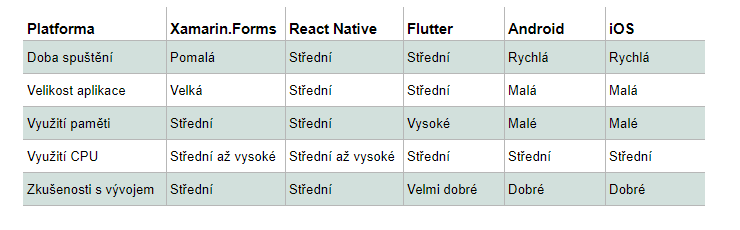
\includegraphics[width=\textwidth]{obrazky/porovnani.png}
\caption{Porovnání vlastností mobilních aplikací vytvořených frameworky a nativními způsoby. \cite{AppsFrameworks}}
\label{fig:frameworks}
\end{figure}

%is by far the most liked cross-platform framework, with 75.4\% of developers
%who are working with Flutter having expressed interest in continuing to use
%it. For React Native, 62.5\% of respondents gave the same answer, and in the
%case of Xamarin, the figure was just 48.3\%. 
\chapter{Použité technologie při tvorbě decentralizovaných aplikací}
\label{chapter:4}
V~následujících sekcích si probereme platformy a frameworky, které velkou mírou přispěli k~vytvoření výsledných aplikací, které jsou dále popsány v~kapitole \ref{chapter:6}.
% přispěly ??
\section{Truffle}
Nástroj Truffle je jedním z~poskytovaných nástrojů v~komplexní sadě Truffle Suite. Uživatelům nabízí vývojové prostředí k~tvorbě smart kontraktů, testovací framework využívající EVM pro jejich následné testování a nakonec příležitost k~nasazení smart kontraktů na sítě Etherea. Ve své práci jsem použil Truffle primárně k~nasazení smart kontraktů na testovací síť Etherea a k~testování smart kontraktů (viz kapitola \ref{chapter:7}). 

V~první řadě je po stažení nástroje nutné si vytvořit projekt příkazem \texttt{truffle init}, který v~aktuální složce utvoří následující strukturu:
\begin{verbatim}
contracts/
migrations/
test/
truffle-config.js
\end{verbatim}
Do složky \texttt{contracts} je potřeba umístit všechny smart kontrakty, které chceme používat. To však neplatí pro importy, které byly staženy pomocí správce balíčků \texttt{npm} nebo \texttt{yarn} do složky s~externími moduly \texttt{node\_modules}. Ve složce \texttt{migrations} mají být uloženy soubory pro migraci. V~ní se mají nacházet javascriptové soubory, podle kterých se provede nasazení smart kontraktů na síť. Jeden soubor zpravidla slouží pro migraci jednoho smart kontraktu a v~případě rozsáhlejšího projektu je nezbytné vytvořit souborů více. Takto vypadá migrační soubor pro hlavní smart kontrakt \texttt{Queans}:

\begin{verbatim}
const Queans = artifacts.require("Queans");

module.exports = function(deployer) {
  deployer.deploy(Queans);
};
\end{verbatim}

Následující složka \texttt{test} může zůstat prázdná. Pokud ale chceme otestovat naše smart kontrakty, tak toto je správné místo pro uložení testů, které jsou napsány opět v~JavaScriptu. Nakonec se dostáváme ke konfiguračnímu souboru \texttt{truffle-config}. Zde si můžeme specifikovat sítě, na které bude náš smart kontrakt nasazen. V~základním nastavení je dostupná síť \texttt{development}, která běží lokálně. Při práci jsem použil testovací síť Etherea Sepolia (viz sekce \ref{sepolia}), které dodávám informace o~poskytovateli a síti. Poskytovatel je zde tvořen pomocí knihovny \texttt{@truffle/hdwallet-provider}, kde je zapotřebí vyplnit klíčovou frázi peněženky, privátní klíč hlavního účtu v~peněžence a URL koncového zařízení, v~našem případě se jedná o~službu Infura (viz sekce \ref{infura}). Adresa prvního účtu v~peněžence je implicitně brána jako tvůrce smart kontraktu. Při správném nastavení se v~této práci smart kontrakt nasadí na síť příkazem \texttt{truffle migrate -{}-network sepolia}. Migrace je provedena na základě všech souborů uložených ve složce \texttt{migrations} \cite{truffle}.
% naše?
\section{Ganache}
Ganache je dalším z~nástrojů dostupných v~sadě Truffle Suite. Jde o~nástroj pro vytvoření osobního blockchainu určeného k~rychlému vývoji aplikací běžících na síti Ethereum. Ganache lze použít dvěma způsoby. Zaprvé jako desktopovou aplikaci, která obsahuje nástroje určené ke sledování stavu sítě, transakcí, bloků a poskytuje i další možnosti pro řízení sítě. Zadruhé ji je možno použít skrze příkazový řádek, který nabízí taktéž plno funkcí, ale již bez pěkného uživatelského rozhraní. 

Při vývoji aplikace jsem používal pouze formu s~příkazovou řádkou, jelikož pro mé základní potřeby byla plně dostačující. Nástroj mi byl nápomocen zejména po úpravě funkcí smart kontraktu k~jejich rychlému otestování pomocí příkazu \texttt{truffle test} (viz kapitola \ref{chapter:7}). V~raných fázích vývoje před připojením na testovací síť Etherea jsem používal používal osobní blockchain taktéž jako testovací síť. 

Po stažení nástroje probíhá spuštění osobního blockchainu v~konzoli pomocí příkazu \texttt{ganache}. Ten vyvolá vytvoření soukromého blockchainu a nabídne uživateli 10 různých účtů včetně testovacích prostředků a privátních klíčů uživatelů. Nasazení smart kontraktu lze docílit příkazem \texttt{truffle migrate -{}-network development} nebo zkráceně \texttt{truffle migrate}, jelikož síť development je brána implicitně. Použití nástroje Truffle je při testování na blockchainu pocházejícího z~Ganache závislé. Pro příkaz \texttt{truffle test} a \texttt{truffle migrate} (platí pouze pro síť development) je nutné mít zapnutý osobní blockchain. Výhodou testovacího prostředí je prakticky neomezený počet prostředků a nepotřebnost konfigurace ostatních souborů \cite{ganache}.
 
\section{Infura}
\label{infura}
Jedná se o~webovou službu, která v~podstatě poskytuje vzdálený uzel Etherea, ke kterému lze přistupovat prostřednictvím rozhraní API. Vývojářům tak umožňuje vytvářet a nasazovat aplikace na hlavní nebo testovací sítě Etherea, aniž by museli provozovat vlastní uzel blockchainu. Při vytvoření účtu si uživatel vytvoří projekt, ke kterému obdrží přidružené Project ID (API klíč).

Tento klíč používám v~zadávání údajů o~poskytovateli v~souboru \texttt{truffle-config}. Po tomto propojení již mohu spustit příkaz \texttt{truffle migrate -{}-network sepolia}, který úspěšně nasadí smart kontrakt na testovací síť Sepolia \cite{infura}.

\section{Sepolia}
\label{sepolia}
Sepolia je jedna ze dvou aktuálně funkčních testovacích sítí Etherea s~cílem napodobovat hlavní síť. Byla navržena tak, aby simulovala náročné podmínky sítě s~rozdílem kratší doby tvorby bloku, což vývojářům umožňuje rychlejší potvrzení transakcí a zpětnou vazbu. Sepolia oproti druhé testovací síti Goerli nabízí dostatek tokenů pro testování a nenastává tak problém s~jejich nedostatkem. Testovací měnu lze získat pomocí tzv. faucetů, kde po zadání adresy účtu uživatel obdrží testovací prostředky. Omezené zdroje získané z~faucetů tak zamezují přetížení sítě \cite{sepolia}.

\section{Expo}
Platforma a open-source framework Expo slouží pro vývoj webových aplikací i mobilních aplikací pro platformy Android a iOS, které běží nativně v~daných systémech. Expo nabízí také mobilní aplikaci Expo Go, která slouží pro testování aplikací React Native, aniž byste museli cokoli lokálně vytvářet. Tato aplikace je rovněž doporučena na oficiálních stránkách React Native pro nové vývojáře mobilních aplikací, díky čemuž jsem ji použil v~průběhu tvorby aplikací. Pomocí Expa lze testovat aplikace buď na fyzickém telefonu nebo s~použitím emulátoru. Aplikaci jednoduše spustíte na počítači příkazem \texttt{npx expo start} a v~případě fyzického telefonu si naskenujete QR kód, který vám v~Expo Go otevře vaši aplikaci. Expo dále nabízí platformu Snack, která dynamicky sestaví a kompiluje kód a funguje jako testovací prostředí, které umožňuje bezprostředně spouštět React Native aplikace v~prohlížeči a poskytuje zobrazení jak na zařízení iOS a Android, ale i pro web. Expo SDK zároveň poskytuje přístup k~mnoha funkcím zařízení a systému, jako fotoaparát, kalendář, kontakty a další. S~pomocí funkce \texttt{EAS Build}, další vychytávkou platformy, je uživatelům umožněno vytvořit produkční sestavu aplikace, která je připravena k~odeslání do obchodů s~mobilními aplikacemi iOS i Android \cite{expo}. 
% aniž byste museli
%aplikaci jednoduše spustíte ... celá věta
% eas build texttt?
\section{Emulátor v~Android studiu}
Android Studio je oficiální integrované vývojové prostředí (IDE) pro vývoj aplikací pro Android. V~našem projektu nás bude zajímat pouze jedna část vývojového prostředí, a to rychlý a funkčně bohatý emulátor, který využijeme namísto fyzického mobilního telefonu se systémem Android. Vývojové prostředí nabízí celou řadu emulátorů s~různými rozlišeními a verzemi operačního systému, díky nimž lze dobře otestovat výslednou aplikaci. 
%citace android studia?
\section{Metamask}
Další potřebnou součástí projektu je kryptoměnová peněženka. Pro své řešení jsem si vybral Metamask, což je softwarová kryptoměnová peněženka, kterou lze nalézt jako webové rozšíření nebo mobilní aplikaci a je stavěna přímo k~interakci se sítěmi Etherea. Kromě toho, že nabízí základní funkce jako jiné peněženky, tak také umožňuje připojení k~decentralizovaným aplikacím a uživatelům tedy umožňuje komunikaci s~blockchainem. Mimo peněženku nabízí Metamask i svůj SDK (Software Development Kit), který nabízí vývojářům jednoduchý způsob propojení aplikací s~peněženkou Metamask \cite{metamask}.
%MetaMask - velké M - opravit všude

\section{Etherscan}
Etherscan je platforma pro Ethereum, která slouží jako prohlížeč blockchainu a zajišťuje spravedlivý přístup k~datům. Díky tomu, že všechny interakce na Ethereu jsou veřejné, prohlížeč nám jednoduše umožňuje je sledovat. Nabízí se nám sledování transakcí, bloků, adres, smart kontraktů a dalších různých dat v~blockchainu \cite{binance_etherscan}. Jeho důležitou rolí je i ověření smart kontraktů, které může jejich autor pomocí zdrojového kódu ověřit. V~ověřených smart kontraktech můžeme vidět jejich zdrojový kód a sledovat, zda se chovají tak, jak mají. Samotné ověření nabízí i jednoduché rozhraní, skrze které lze otestovat chování smart kontraktů bez použití decentralizovaných aplikací \cite{etherscan}.

\chapter{Současný stav Q\&A řešení}
\label{chapter:5}
Tato kapitola má za cíl krátce objasnit pojem Q\&A sekce společně s~možnostmi výběru otázek v~médiích a v~další řadě přiblížit aplikace nabízející Q\&A sekci. Na konci kapitoly provedu kritické zhodnocení zmíněných aplikací a návrh, jak se zmíněným nevýhodám existujících řešení vyvaruji v~samotné práci. 
% vyvaruji
\section{Q\&A sekce}
Sekcí otázka/odpověď rozumíme prostor, kde lidé mohou klást otázky, na které chtějí získat odpovědi. Obecně se může jednat o~interaktivní dialog mezi hostem, případně moderátorem, a publikem \cite{slidoqa}. Během relace mohou diváci nebo posluchači pokládat své otázky, které jsou následně zodpovězeny. Cílem těchto relací je umožnit divákovi nebo posluchači možnost aktivně se zapojit do diskuze a získat dodatečné informace o~dané problematice. Nejčastěji jde o~otázky relevantní pro dané programy a často se týkají aktuálních událostí, ať již politických, kulturních nebo sportovních. Tento formát se mnohdy využívá v~talk show, rozhovorech, panelových diskuzích nebo při přednáškách. V~této práci bych se chtěl zaměřit na televizní a rozhlasové relace, kde vidím největší přínos aplikace. 
% otázka/odpověď
\subsection*{Výběr otázek v~médiích}
Způsob výběru otázek se samozřejmě může lišit a záleží jen na konkrétní relaci a pořadateli, jak k~výběru přistoupí. V~každém případě by měla být zajištěna transparentní a férová selekce otázek. Díky ní publikum obdrží odpověď na to, co si žádá. Bohužel nelze zaručit, že dotazy nebudou žádným způsobem cenzurovány ani zmanipulovány. Níže jsou popsány 3 způsoby, jak média přistupují k~výběru otázek.
\begin{enumerate}
\item Předem zvolené otázky: Pořadatelé si před začátkem relace sestaví seznam otázek, které host zodpoví. Výběr konkrétních otázek se děje na základě předem definovaných kritérií, jimiž jsou aktuálnost tématu, relevance pro publikum či nápaditost.
% které host zodpoví?
\item Předem získané otázky publika: Posluchači a diváci jsou před začátkem relace osloveni, aby zaslali své otázky skrze sociální média nebo e-mail. Pořadatelé následně vybírají ty, které subjektivně vyhodnotí jako nejlepší či nejvhodnější.

\item Živé otázky: Během probíhající relace je umožněno jejímu publiku pokládat otázky živě nebo pomocí mobilního telefonu (ať již telefonátem nebo zprávou), chatu či jiné platformy. Moderátor následně vybírá otázky, které budou zodpovězeny. 
\end{enumerate}

\section{Analýza současných Q\&A aplikací}
\label{analyza}
\begin{figure}[h]
\centering
\begin{minipage}{.5\textwidth}
  \centering
  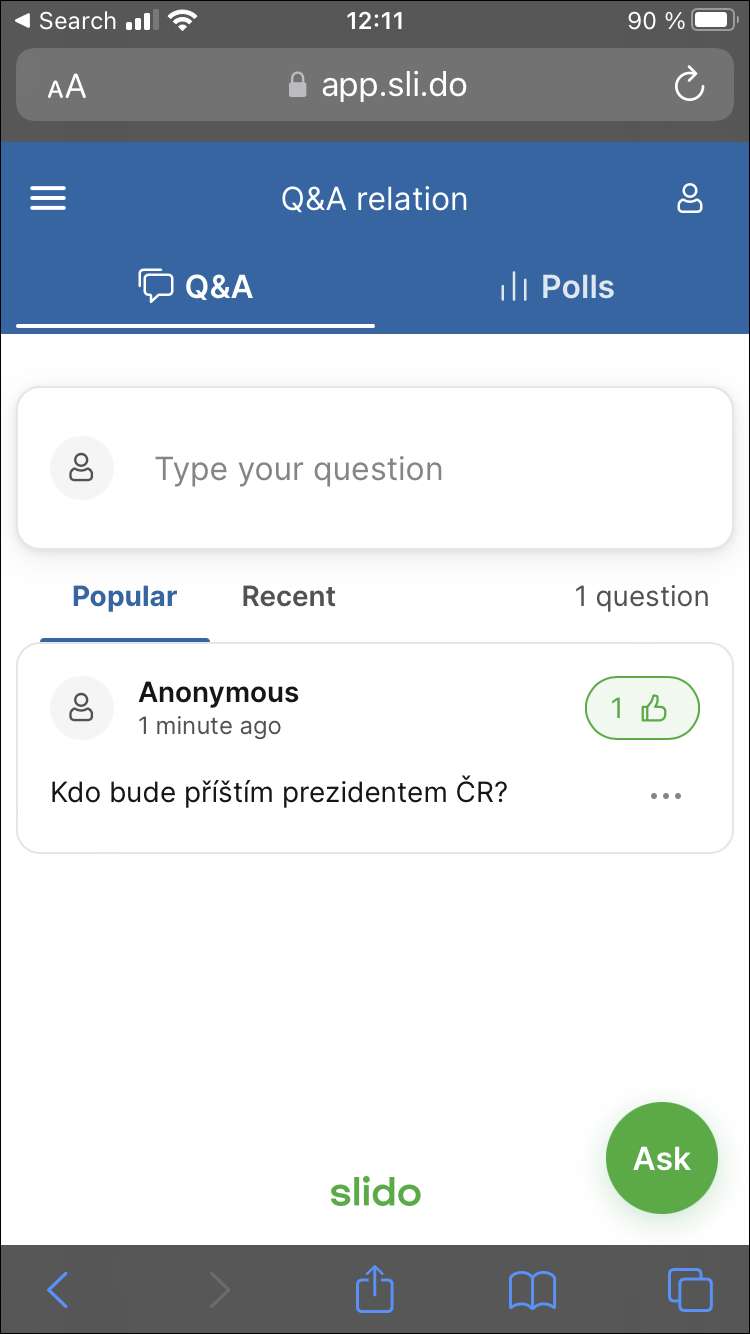
\includegraphics[width=.9\linewidth]{obrazky/slido_client.png}
  \captionof{figure}{Slido - pohled uživatele}
  \label{fig:sub1}
\end{minipage}%
\begin{minipage}{.5\textwidth}
  \centering
  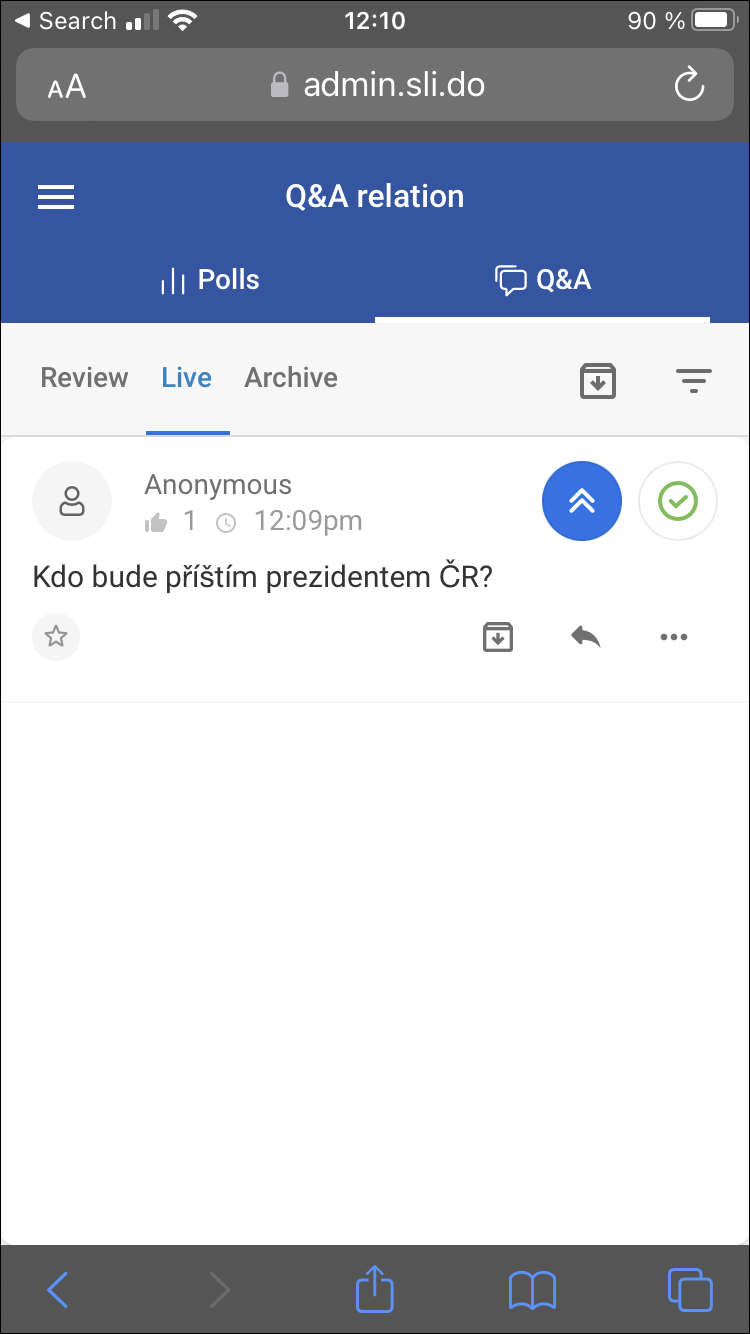
\includegraphics[width=.9\linewidth]{obrazky/slido_admin.png}
  \captionof{figure}{Slido - pohled přednášejícího}
  \label{fig:sub2}
\end{minipage}
\end{figure}

\subsection{Slido}
Jedná se o~online aplikaci pro interakci mezi účastníky a přednášejícími, která se používá zejména při přednáškách, prezentacích, workshopech, konferencích a dalších podobných akcích. Aplikace nabízí různou paletu nástrojů, avšak my se zaměříme pouze na jednu její část - sekci otázek a odpovědí. Slido umožňuje jednoduše zadávat otázky po naskenování QR kódu nebo po zadání hesla pro konkrétní relaci \cite{slidosection}. Na obrázcích \ref{fig:sub1} a \ref{fig:sub2} jsou zobrazeny náhledy webové aplikace na mobilním telefonu z~pohledu uživatele i přednášejícího.

Diváci nemají žádné omezení na počet otázek, který mohou položit a jsou schopni jakoukoliv z~vlastních otázek během 5 minut od jejího položení editovat. Vzájemně mají prostor k~hlasování pro otázky druhých. Tímto způsobem je zajištěna dynamika pořadí nejoblíbenějších otázek. Zobrazení dotazů je možné dvěma způsoby, a to podle popularity otázek nebo podle času, kdy byly zadány. Publikum si dále může vybrat, zda chce položit dotazy buď anonymně nebo pod jménem, které zadají. Ze strany účastníka jsme tímto zmínili všechny jeho možnosti, které jsou pro Q\&A sekci nabídnuty.  
% které zadají
Nyní se přesuneme na stranu organizátora Q\&A sekce, která je už poněkud obsáhlejší. Ten má možnost otázky označit jako oblíbené, zodpovězené (otázka se následně archivuje a publiku již není dostupná) nebo zvýraznit konkrétní otázku ve chvíli, kdy na ni odpovídá. Dále má příležitost jakoukoliv otázku upravit (po editaci se zobrazí text oznamující úpravu otázky, kde ale není zřejmé, jestli proběhla uživatelem nebo organizátorem), textově na ni odpovědět, archivovat nebo smazat. Slido nabízí další dodatečné funkce, jako jsou exporty otázek, různé souhrny nebo i variantu, ve které se nejprve dotaz odešle ke schválení organizátorovi, který podle jeho obsahu uzná za vhodné, zda dotaz zveřejnit. Část z~vyjmenovaných funkcí je ale podmíněna placeným měsíčním členstvím, které ale naštěstí není požadované pro vytvoření Q\&A sekce.

\begin{figure}
\centering
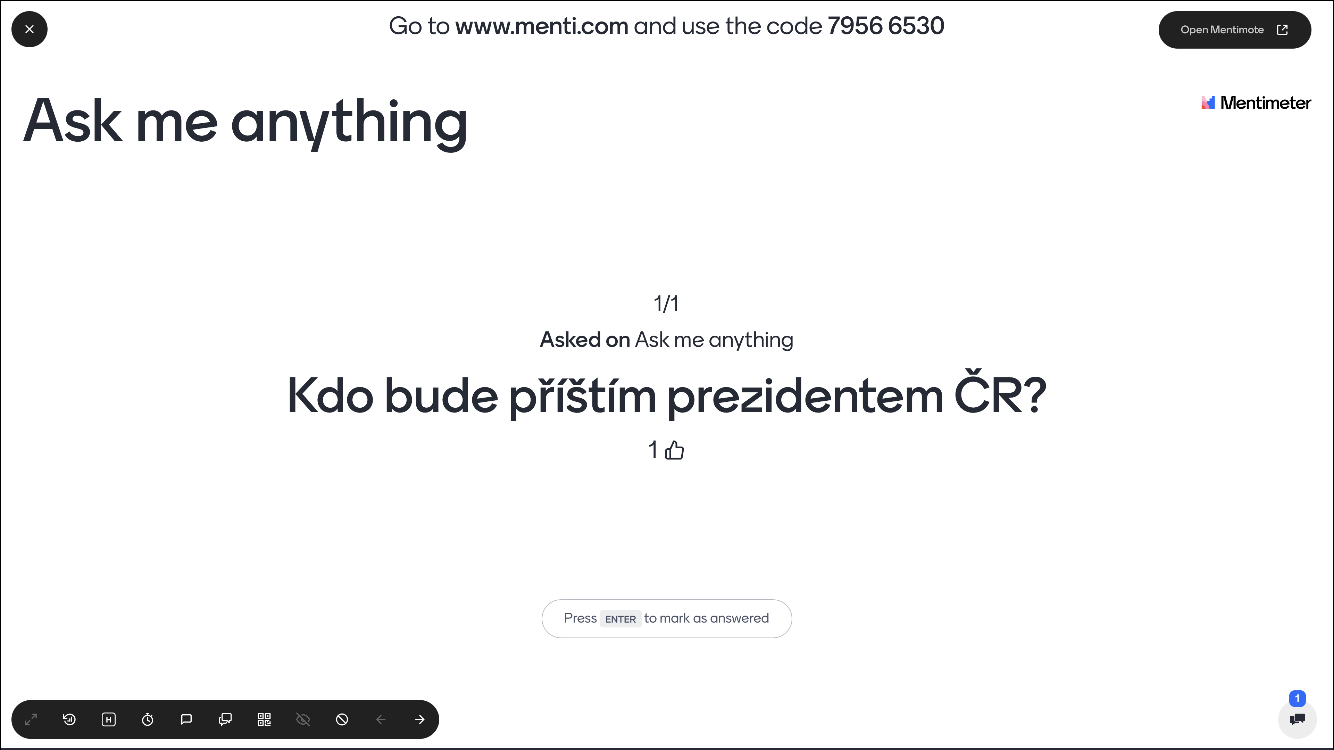
\includegraphics[width=.9\linewidth]{obrazky/mentimeter_admin.png}
\caption{Mentimeter - pohled prezentujícího, širokoúhlé zobrazení}
\label{fig:sub3}
\end{figure}

\begin{figure}
\centering
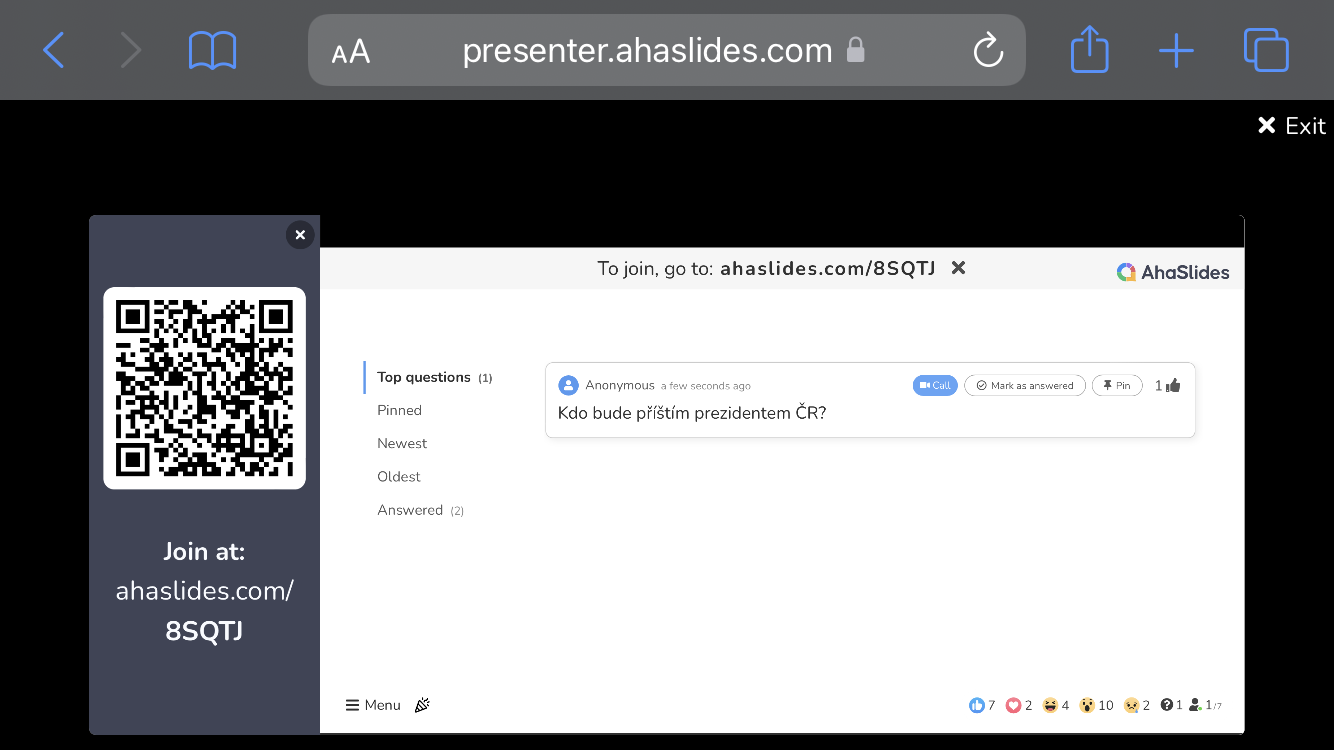
\includegraphics[width=.9\linewidth]{obrazky/aha_admin.png}
\caption{AhaSlides - pohled prezentujícího, širokoúhlé zobrazení}
\label{fig:sub4}
\end{figure}

\begin{figure}
\centering
\begin{minipage}{.5\textwidth}
  \centering
  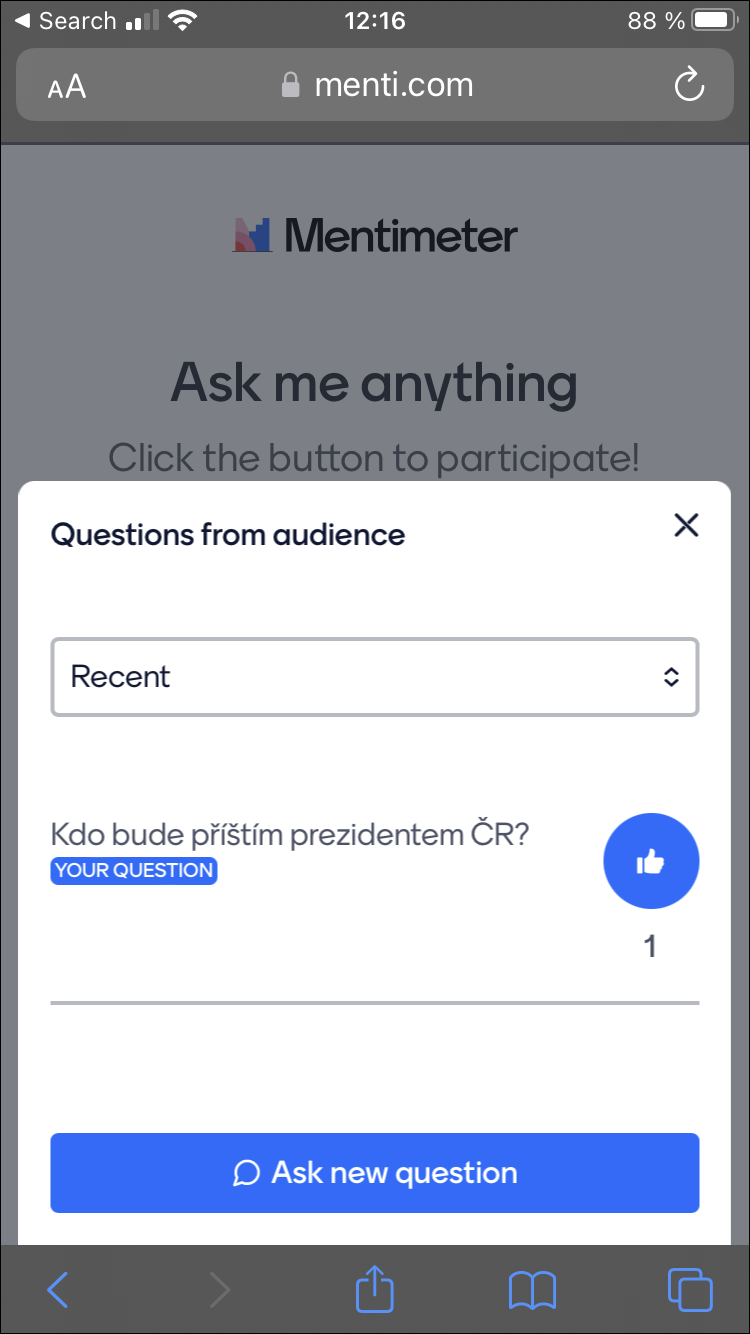
\includegraphics[width=.7\linewidth]{obrazky/mentimeter_client.png}
  \captionof{figure}{Mentimeter - pohled uživatele}
  \label{fig:sub5}
\end{minipage}%
\begin{minipage}{.5\textwidth}
  \centering
  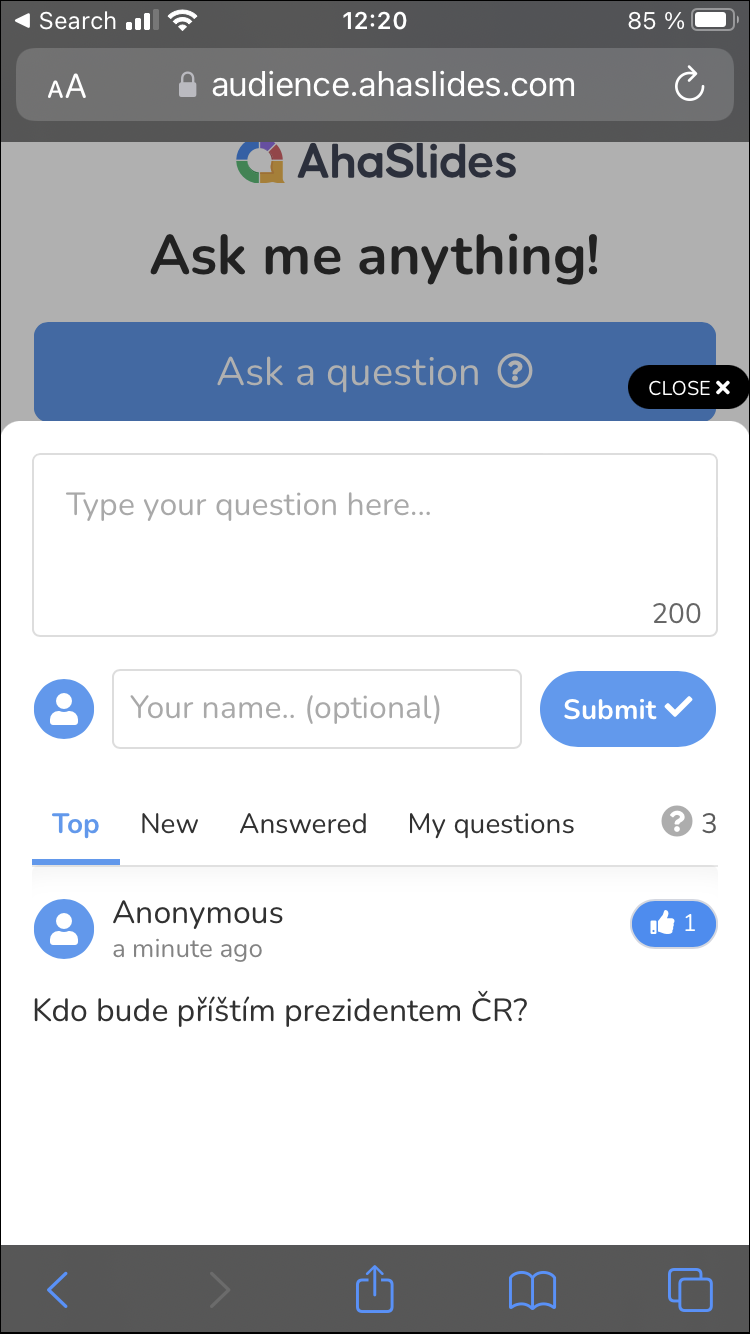
\includegraphics[width=.7\linewidth]{obrazky/aha_client.png}
  \captionof{figure}{AhaSlides - pohled uživatele}
  \label{fig:sub6}
\end{minipage}
\end{figure}

\subsection{Mentimeter}
Mentimeter je jedna z~řady webových aplikací, která umožňuje založit Q\&A sekci při prezentaci. Využívá se především v~průběhu nebo na konci přednášek s~prezentací, kde se na snímku zobrazí výčet dotazů, na které chce publikum znát odpověď. Mentimeter nabízí několik různých druhů snímků pro sestavení prezentace. Do sekce se účastník dostane pomocí naskenování QR kódu nebo zadáním 8 místného hesla \cite{mentimetersection}. Na obrázcích \ref{fig:sub3} a \ref{fig:sub5} je znázorněno zobrazení aplikace na mobilním zařízení. 

Uživatelské rozhraní je minimalistické a nabízí jen několik málo možností, jak s~otázkami nakládat. Dotazy lze položit pouze anonymně, nikoliv pod konkrétním jménem. 
Diváci mají příležitost hlasovat pro otázky, které se jim líbí. Nakonec si mohou urovnat pořadí otázek buď podle počtu hlasů nebo podle času, kdy byly vytvořeny.

Samotný moderátor před začátkem prezentace nastavuje, zda publikum může pokládat otázky na všech druzích snímků nebo pouze na snímcích označených jako Q\&A. Dále je schopen nastavit, jestli ostatní účastníci vidí dotazy ostatních. V~případě, že nevidí, nelze pro žádné hlasovat. Při prezentaci je prezentujícímu umožněno označit otázky za zodpovězené nebo je odstranit. Placený plán nabízí volbu, při které lze dotazy schvalovat ještě před tím, než jsou zobrazeny ostatním.

\subsection{AhaSlides}
Poslední aplikací, kterou si popíšeme, je AhaSlides. Organizátorům poskytuje možnost vytvoření prezentace, ve které lze použít Q\&A snímky \cite{ahasection}. Jedná se o~velice podobnou alternativu k aplikaci Mentimeter. Po naskenování QR kódu nebo použitím speciálního odkazu se uživateli zobrazí pohled z~obrázku \ref{fig:sub6}.

Rozhraní dovoluje uživateli pokládat otázky pod zvoleným jménem, které se zadává pro každou otázku zvlášť nebo anonymně. Publikum má příležitost hlasovat pro otázky ostatních, aby se dostaly na lepší pozici a zvýšila se šance na zodpovězení. Poslední možností je opět srovnání dotazů podle jejich hodnocení nebo času, kdy byly položeny.
% nebo anonymně - čárka před?
% šance na JEJICh zodpovězení?
Prezentující má možnost otevřít další okno pro moderátora, který může přicházející dotazy před zveřejnením schvalovat nebo zamítnout. Dále může otázky třídit do následujících kategorií: nejlepší otázky, označené, nejnovější, nejstarší a zodpovězené. AhaSlides také nabízí filtrování explicitních výrazů a možnost zavolat autorovi konkrétní otázky. Jeho pohled je znázorněn na obrázku \ref{fig:sub4}.

\section{Porovnání existujících aplikací s~cíli stanovenými pro tuto práci}
Jak jste mohli vidět, existuje několik aplikací pro vytvoření Q\&A sekce. Další z~těch, které tu nebyly zobrazeny, fungují na velice podobném principu jako Mentimeter či AhaSlides a jejich použití je optimalizováno na prezentace ve školách nebo při přednáškách. Všechny tři aplikace jsou vytvořeny jako webové, přičemž Mentimeter a AhaSlides jsou vytvořeny z~pohledu prezentujícího výhradně pro počítač a v~mobilním zobrazení nejsou responzivní. Jejich ovládání je na telefonu poněkud složité z~důvodu malých tlačítek, a to i při širokoúhlém zobrazení. Po vyzkoušení aplikací a zamyšlení se, proč neexistují v~podobě mobilních aplikací, jsem došel k~závěru, že není optimální aplikaci stahovat, zejména pokud je nedostatek času. Zkrátka jednodušším řešením je načíst webovou aplikaci, připojit se a rovnou se zapojit do komunikace. Výjimku zde tvoří Slido, které nabízí mobilní aplikaci, ale pouze pro publikum, ve které však bohužel nevidím oproti webové variantě žádný přínos a označil bych ji tak za téměř zbytečnou. Slido oproti dvěma zbylým variantám nabízí jednoduché a přehledné rozhraní pro přednášející i na samotném telefonu. Z~pohledu účastníka jsou všechny tři varianty velice podobné a uživatelsky přívětivé.  
% TODO
% jak jste mohli vidět - JAk jste si mohli přečíst?

Postoupíme-li o~krok dále a zaměříme-li se na decentralizované aplikace, musím konstatovat, že jsem nebyl schopen žádnou decentralizovanou aplikaci, která by nabízela Q\&A sekci vyhledat. 
% TODO 
% sekci vyhledat - čárka?
Nyní si rozebereme jednotlivé nevýhody, které existujicí řešení obsahují. První z~nich je samotná cenzura. Všechna tři řešení nabízí omezování dotazů několika různými způsoby. Jedním je příležitost kontrolovat příchozí otázky a na základě jejich obsahu je schválit nebo odstranit, případně s~nimi nic nedělat. V~případě Slida se jedná ještě o~další možnost, kterou je editace zpráv. Po změně zprávy se označí jako \uv{edited} a žádný z~uživatelů nemá šanci zjistit, zda ji změnil sám autor nebo organizátor. Druhou nevýhodou označíme příležitost ke spamu. Pokud pomineme možnosti, že lze omezit celé publikum, aby nemohlo pokládat otázky, a kontrolu příchozích otázek, nastává riziko, že se do relace dostane nechtěný účastník, který ji bude zahlcovat velkým množstvím dotazů. I~přes kontrolu příchozích otázek může toto chování organizátorům velice znepříjemnit průběh relace.
% TODO_HM 
% edited - dal jsem uvozovky - asi upravit jinak?
% jedním z nich
Jak je zmíněno již v~kapitole \ref{chapter:1}, aplikace by mohla mít své využití ve veřejnoprávních médiích, ale i všude, kde chceme zaručit transparentnost samotného procesu dotazování se skrze online prostor. Dvě nevýhody, které jsme zmínili v~předešlém odstavci, se snaží má práce odstranit. Neschopnost cenzury otázek a její ověření bude umožněno díky vlastnostem blockchainu, transparentnosti smart kontraktu a aplikaci, která slouží jako rozhraní, skrze které nebude nikdo schopen jakkoli omezovat publikum relace. Druhou, neméně důležitou problematiku spamu znemožní maximální možný počet otázek, který může uživatel přispět do relace. Aktuálně je tento počet nastaven na hodnotu 1. Dalším pomocníkem je smart kontrakt určený ke správě identit, který dovolí se do relace dostat pouze pod podmínkou, že uživatel prokáže správci identit svoji identitu. V~aplikaci je tento způsob pouze simulací reality, nicméně při reálném provozu by se předpokládalo například předložení bankovní identity nebo občanského průkazu k~ověření identity uživatele.
% které jsme zmínili - teré jsem zmínil?
% který může uži - kterým?
%a aplikaci, která slouží? je to tak?
\chapter{Návrh a implementace}
\label{chapter:6}
Na následujících stránkách si nejprve představíme návrh aplikace a uvedeme protokol pro pro decentralizované řízení Q\&A sekcí. Dále si popíšeme, jaké hlavní funkce poskytují smart kontrakty \texttt{identityRegistry} a \texttt{Queans}. Nejdříve se pojďme podívat, jak by mohla výsledná aplikace vypadat.  

\section{Návrh aplikace}
Při návrhu je nejdůležitější si rozmyslet, co a kde bude umístěno a jak by se mělo co chovat. Zde se mi nabízely 2 způsoby řešení. Jedním z~nich bylo vytvořit jednu aplikaci, ve které si lze vybrat, zda chce být uživatel moderátorem nebo běžným účastníkem relace. Druhý způsob nabízel tvorbu dvou aplikací, kde první by byla pro publikum relací a druhá čistě pro moderátory. Na obrázcích \ref{fig:navrh1} a \ref{fig:navrh2} je prvotní návrh samostatné aplikace. Nakonec jsem se však vydal opačnou cestou, přestože dlouhou dobu to vypadalo, že bude vyhovující pouze jedna aplikace. Postupem času se ale smart kontrakt \texttt{Queans} měnil a s~ním i podoba aplikace. 

Dále jsem vytvořil třetí aplikaci nad rámec práce, která představuje proces ověřování u~poskytovatele identit. V~původním návrhu měly být identity ověřeny pouze skrze tlačítko \texttt{verify user} podle obrázku \ref{fig:navrh1}, kde by se ověřil aktuálně přihlášený uživatel, který by následně mohl využívat aplikaci. Aplikace využívá smart kontrakt \texttt{identityRegistry} popsaný v~sekci \ref{identityRegistry}.

Mým cílem bylo vytvořit všechny aplikace nabízející rozhraní, které bude mít základní funkcionalitu, ale bude plně funkční. První aplikace s~pracovním názvem Voter slouží pro běžné uživatele. Druhá má název Moderator a je využita výhradně moderátory relací. Poslední z~nich se nazývá Management a slouží pro správu identit uživatelů.
K~interakci s~blockchainem slouží 2 hlavní smart kontrakty. Prvním je již zmiňovaný \texttt{identityRegistry}, který rozšiřuje rozhraní \texttt{IIdentityRegistry} a používá smart kontrakty \texttt{MultisigAction\-Members} a \texttt{MultisigMembers}. Druhým je smart kontrakt \texttt{Queans} popisovaný v~sekci \ref{queans}, který jsem vytvořil jako součást práce. 

\begin{figure}
\centering
\begin{minipage}{.5\textwidth}
  \centering
  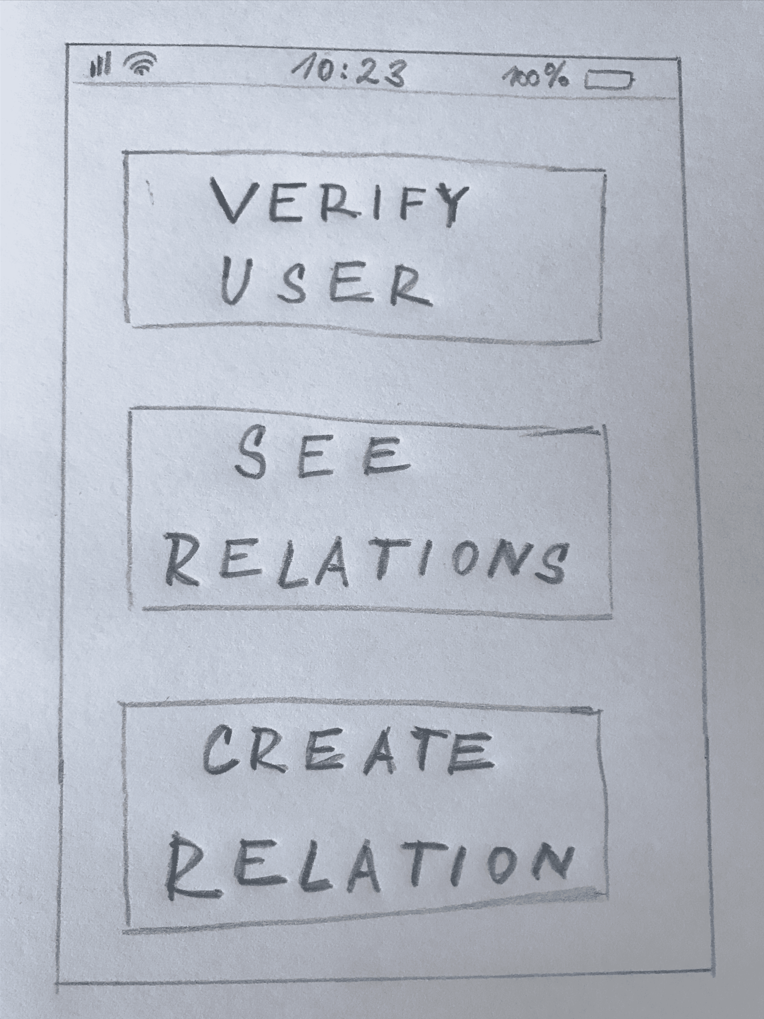
\includegraphics[width=.9\linewidth]{obrazky/Navrh_uvod.png}
  \captionof{figure}{Návrh úvodní obrazovky}
  \label{fig:navrh1}
\end{minipage}%
\begin{minipage}{.5\textwidth}
  \centering
  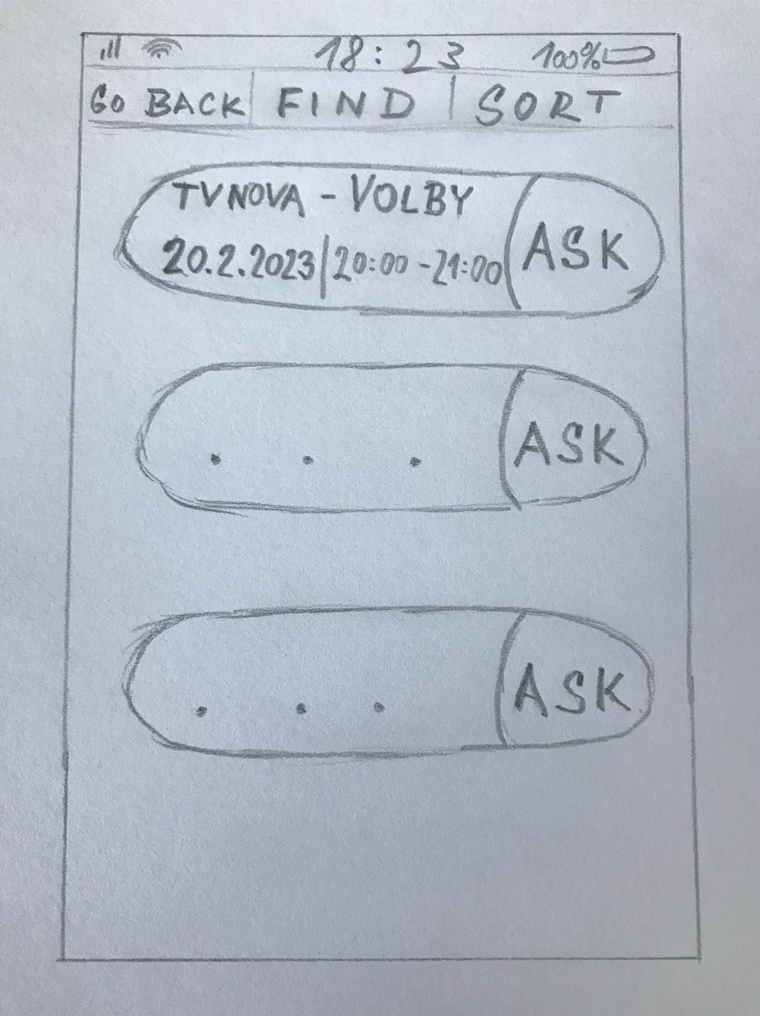
\includegraphics[width=.9\linewidth]{obrazky/Navrh_prehled.png}
  \captionof{figure}{Návrh přehledu relací}
  \label{fig:navrh2}
\end{minipage}
\end{figure}

\section{Návrh protokolu vhodného pro decentralizované řízení Q\&A sekcí}
\label{protokol}
Před samotnou implementací smart kontraktu zajišťujícího decentralizované řízení Q\&A sekcí bylo třeba navrhnout protokol, podle kterého se bude implementace řídit. Návrh protokolu je popsán na obrázku \ref{fig:protokol}. Jak si můžete všimnout, je tvořen 5 základními entitami a 4 fázemi a entita blockchain v~protokolu zahrnuje všechny smart kontrakty, které aplikace používá. 
% a entita - kde entita?
V~první fázi se vyskytují administrátor správy identit, poskytovatel identit a uživatel. Administrátor je osoba, případně skupina osob, která je zodpovědná za přidávání nových poskytovatelů identit (angl. identity providers, zkr. IDP) na základě jejich digitální identity. Poskytovatelé identit mají za úkol ověřovat identitu poskytnutou od uživatelů (v~případě této práce jde o~blockchainovou adresu uživatele) a následně přidat ověřené uživatele do smart kontraktu. Všechny funkce první fáze jsou implementovány v~aplikaci s~názvem Management.  

Druhá a třetí fáze je implementovaná v~aplikaci pro moderátory. Druhá fáze zobrazuje proces tvorby relace a změnu uživatele na moderátora. Ve třetí fázi dochází k~přípravě relace na hlasování. Zde může moderátor zvát do soukromé relace účastníky a následně změnit stav relace, aby mohla začít poslední fáze. 

Ve čtvrté fázi již figuruje pouze uživatel, který může pokládat otázky do různých relací a hlasovat pro otázky ostatních uživatelů. Tato fáze je implementovaná v~aplikaci Voter.

\begin{figure}
\centering
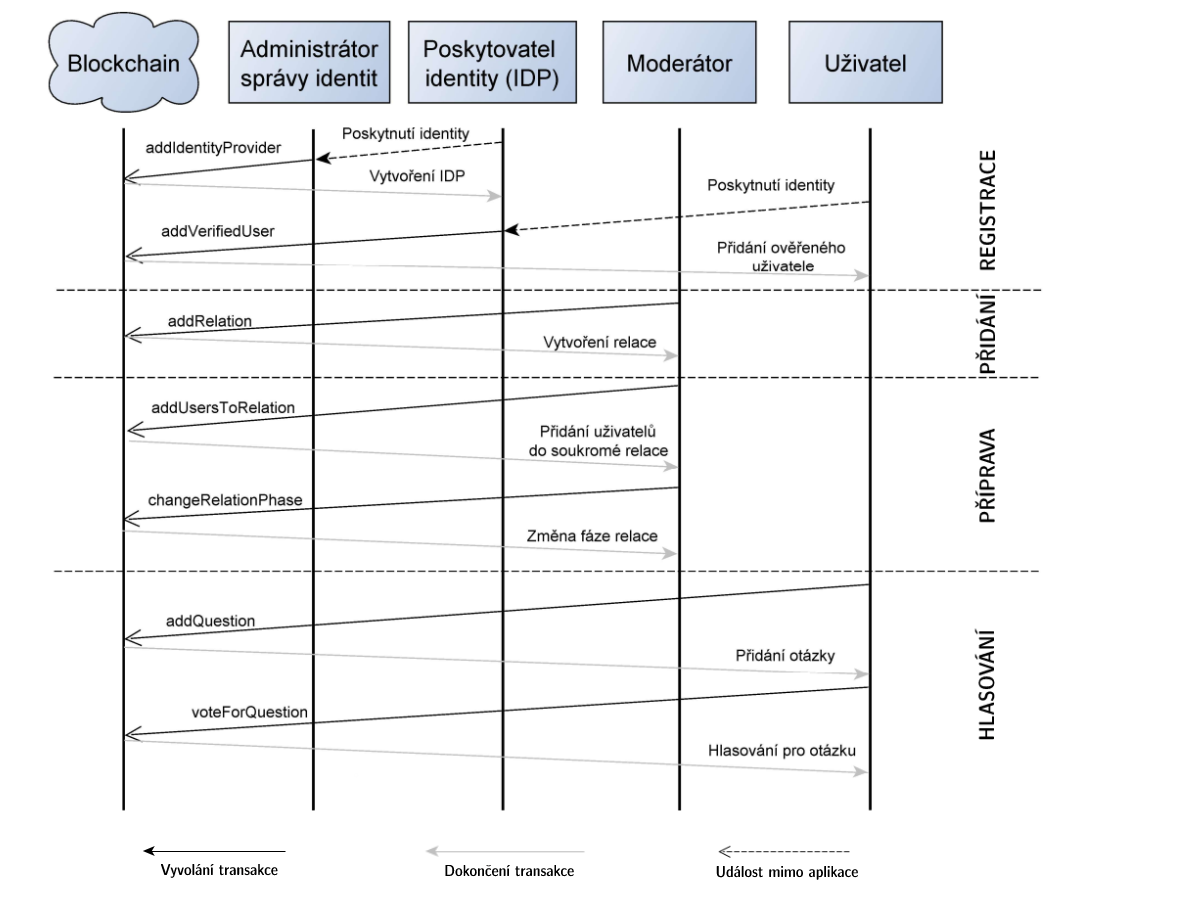
\includegraphics[width=\linewidth]{obrazky/protokol_sipky.png}
\caption{Protokol komunikace}
\label{fig:protokol}
\end{figure}
\subsection*{Motivace uživatelů}
Čím jsou uživatelé, kteří se podílejí svoji účastí v~relaci, motivováni? Pokud už se někdo do relace připojí, nejspíše tak jedná za účelem se pobavit nebo se dozvědět nové informace. Většina nepředpokládá, že by za svoji účast mohla být odměněna ještě jiným způsobem, přestože organizátoři některých akcí oceňují aktivní publikum dárky. V~našem případě by těmito \uv{dárky} mohla být finanční odměna v~podobě mincí nebo tokenů sítě, na které by byl smart kontrakt spuštěn. Implementaci jsme se rozhodli s~vedoucím práce nedělat, ač by nemusela být příliš složitá. Pokusím se tedy nastínit nápady, které by mohly být v~rozšíření aplikace uskutečněny. Po ukončení relace je možné odměnit otázku s~nejvíce hlasy určitým poměrem získaných prostředků stanoveným podle počtu celkových otázek dané relace. Stejným způsobem by se dalo ocenit i nejlepších \uv{X} otázek, jen by se upravil poměr odměn za jednotlivá místa. Další možností je ohodnotit i tvůrce samotné relace, a to za aktivitu uživatelů, kteří platí poplatky za pokládání dotazů a hlasování. Další možností je i označení aktivních účastníků relací v~samotné aplikaci, aby dali ostatním najevo, že jsou po dlouhou dobu nedílnou součástí relací.  
% TODO
% většina nepředpokládá?
% TODO_HM 
% mplementaci jsme se rozhodli? 
%pokud už se někdo - pokud se už 
mohly být
\section{identityRegistry}
\label{identityRegistry}
Tato sekce se zabývá smart kontraktem \texttt{identityRegistry}, který mi byl poskytnut k~použití vedoucím práce doktorem Homoliakem, stejně jako smart kontrakty \texttt{MultisigAction\-Members} a \texttt{MultisigMembers} a rozhraní \texttt{IIdentityRegistry}. Jedná se o~smart kontrakt, ve kterém se vyskytují 3 typy entit a slouží zejména k~ověření identit uživatelů. Entitami jsou administrátoři správy identit (zkr. IDM admin), poskytovatelé identit (zkr. IDP, angl. identity provider) a uživatelé, kteří chtějí ověřit svoji identitu. Níže si popíšeme tři nejdůležitější funkce, které jsou využity ve výsledných aplikacích. Po nasazení smart kontraktu máme pouze administrátora, kterým se stane osoba, která ho nasadila na síť. 
% IDP opakuje se - smazat
% 3 nejdůležitější funkce - smart kontraktu
\subsection{funkce addIdentityProvider}
První funkcí, kterou si zmíníme, je funkce sloužící k~přidání poskytovatele identity. K~vytvoření nového poskytovatele identity je potřebné zadat jeho adresu, digitální identitu a jméno, jak je zobrazeno na obrázku \ref{fig:idp1}. Funkci může provádět výhradně administrátor správy identit. V~případě, že by administrátorů bylo více, musí nadpoloviční většina schválit přidání konkrétního poskytovatele identity. Pro zjednodušení funkčnosti aplikace však nelze v~rozhraní výsledné aplikace další administrátory přidávat. 
%TODO_HM 
% adresa - blockchainova adresa?

\subsection{funkce addVerifiedUser}
Nyní přejdeme k~funkci, která se stará o~přidávání ověřených uživatelů do smart kontraktu. Za tuto činnost jsou zodpovědni poskytovatelé identity, jejichž úkolem je ověřovat uživatele na základě jimi poskytnuté identity a následně je buď zařadit nebo nezařadit mezi ověřené uživatele ve smart kontraktu. Pro provedení operace využívají rozhraní zobrazené na obrázku \ref{fig:idp2}, kde poskytovatel identity vyplňuje svůj privátní klíč, svoji veřejnou adresu a adresu uživatele. Pomocí privátního klíče se podepisuje adresa uživatele s~textovým řetězcem a adresou smart kontraktu. Ve funkci \texttt{addVerifiedUser} se následně porovná pomocí funkce \texttt{ecrecover} veřejný klíč s~podpisovými daty, který slouží ke kontrole, že operace byla provedena autorizovanou osobou. 
% TODO 
% jimi?
\begin{figure}
\centering
\begin{minipage}{.5\textwidth}
  \centering
  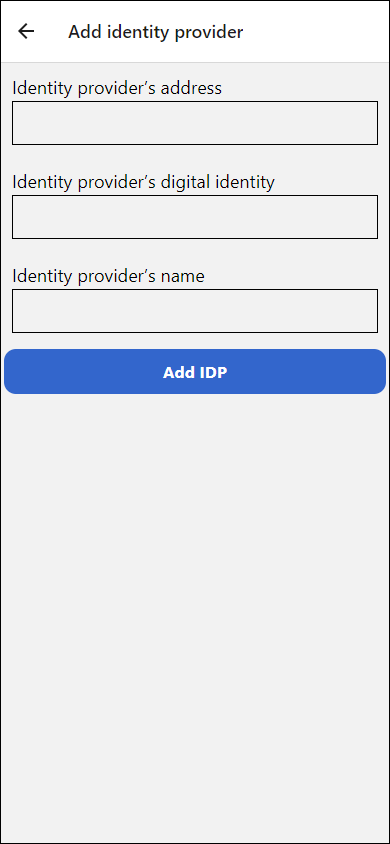
\includegraphics[width=.9\linewidth]{obrazky/idp1.png}
  \captionof{figure}{Rozhraní aplikace znázorňující \newline přidání nového poskytovatele identity}
  \label{fig:idp1}
\end{minipage}%
\begin{minipage}{.5\textwidth}
  \centering
  
\includegraphics[width=.9\linewidth]{obrazky/idp2.png}
  \captionof{figure}{Rozhraní aplikace znázorňující \newline přidání ověřeného uživatele}
  \label{fig:idp2}
\end{minipage}
\end{figure}

\subsection{funkce verifyIdentity}
Nakonec se dostáváme k~externí funkci, jejíž úkolem je potvrdit, že identita uživatele (v~našem případě adresa), již byla ověřena poskytovatelem identity. Funkce se volá přes rozhraní \texttt{IIdentityRegistry}, jehož funkce je specifikována ve smart kontraktu \texttt{identityRegistry}. V~konstruktoru smart kontraktu \texttt{Queans} je napevno nastavena adresa smart kontraktu \texttt{identityRegistry} a přiřazena do inicializovaného rozhraní. \texttt{VerifyIdentity} ověřuje adresu odesílatele blockchainové transakce a používá se ve všech funkcích smart kontraktu \texttt{Queans}, které mění stav blockchainu (smart kontraktu). Tímto způsobem je demonstrováno ověření identit třetí stranou (jiným smart kontraktem).
% TODO_HM 
% adresa - blockchainová adresa
\section{Queans}
\label{queans}
V~této sekci se podíváme na smart kontrakt \texttt{Queans}, který byl jednou ze dvou hlavních částí práce. \texttt{Queans} je naprogramován podle protokolu v~sekci \ref{protokol} a tvoří jádro samotné aplikace. Níže si podrobně povíme o~uživatelích, relacích a otázkách.

\subsection{Uživatelé}
Uživatelé jsou nedílnou součástí většiny aplikací. I~v~našem případě tomu tak je. Mezi uživatele se z~protokolu na obrázku \ref{fig:protokol} řadí kromě jich samotných i moderátor, který je speciálním typem uživatele. Moderátorem se stane tak, že vytvoří relaci, ve které získá roli moderátora, nicméně ve všech ostatních relacích je pouhým uživatelem. Abychom mohli pracovat s~jejich adresami, bylo nutné si vytvořit datovou strukturu, kde budou uloženy. Tou je množina adres přejatá z~knihovny \texttt{@openzeppelin}. 
%uloženy? uloženi?
\subsubsection{EnumerableSet.AddressSet users}

Oproti klasickému poli se jedná o~optimalizovanou strukturu pro ukládání jednoho typu hodnot, v~našem případě adres, která ještě navíc nabízí funkci \texttt{contains()} pro ověření, zda se konkrétní prvek nachází v~dané množině. Do množiny se uživatel dostane automaticky po použití jedné z~funkcí měnících stav blockchainu (smart kontraktu). Podmínkou však je, že byl již dříve ověřen poskytovatelem identity. 

\subsection{Relace}
Po uživatelích jsou relace jako druhá nejdůležitější část kontraktu. Nejprve si zobrazíme strukturu relace a povíme si o~jejích nejdůležitějších částech. 

\begin{verbatim}
struct Relation {
    address author;
    uint creationTime; 
    bool isPublic; 
    bool votePhase; 
    address[] privateList; 
    uint ID;
    uint startOfRelation; 
    uint questionCloseTime; 
    string name; 
    uint[] questionsKeys;
}
\end{verbatim}

Většina částí tvořících relaci je nezajímavých a od založení relace se nemění. Nicméně bych rád vyzdvihl čtyři z~nich, které značně ovlivňují fungování celé aplikace. První je proměnná \texttt{isPublic}. Ta udává, zda je relace otevřená všem uživatelům nebo je omezená pouze pro pozvané účastníky. S~tím se pojí i pole \texttt{privateList}, které v~sobě uchovává adresy všech pozvaných uživatelů do relace. V~případě, že je relace veřejná, pole \texttt{privateList} zůstane prázné a nepracuje se s~ním. Jestliže ale moderátor nastaví relaci jako soukromou, musí také přidat účastníky za pomoci funkce \texttt{addUsersToRelation}, aby se někdo mohl relace zúčastnit. Další důležitou proměnnou je \texttt{votePhase}, jež nám udává fázi konkrétní relace. \texttt{VotePhase} při hodnotě \texttt{false} znamená, že hlasovací fáze relace ještě nezačala a tento stav nazývám v~aplikaci jako \uv{preparation}. Změna je pouze jednorázová, tudíž si musí moderátor rozmyslet, v~jaký okamžik relaci přepne. V~přípravné fázi lze pouze zvát uživatele do relace a případně si zobrazit, koho už autor pozval. V~hlasovací fázi je již umožněno pozvaným účastníkům pokládat otázky a hlasovat pro otázky druhých. Poslední nezbytnou částí relace je pole čísel \texttt{questionKeys}, které uchovává ID jednotlivých otázek, čímž získáme přehled o~všech otázkách relace, kterými uživatelé přispějí.
% TODO_HM 
% a tento stav nazývám v aplikaci jako „preparation“ možná do texttt - dal jsem uvozovky ??
\begin{figure}
\centering
\begin{minipage}{.5\textwidth}
  \centering
  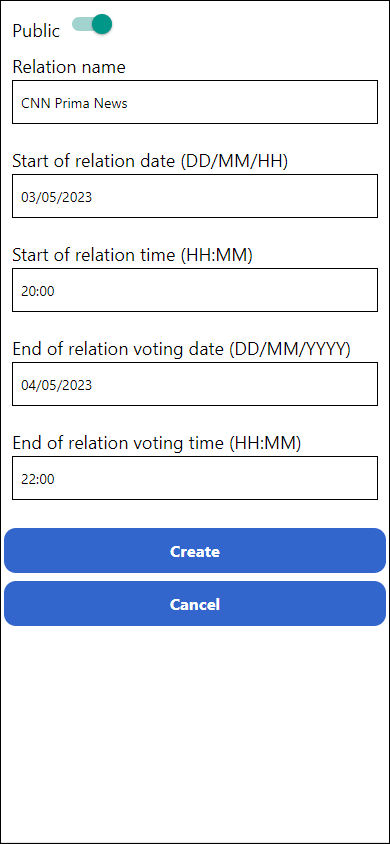
\includegraphics[width=.9\linewidth]{obrazky/pridat_relaci.png}
  \captionof{figure}{Rozhraní aplikace pro \newline vytvoření nové relace}
  \label{fig:pridani_relace}
\end{minipage}%
\begin{minipage}{.5\textwidth}
  \centering
  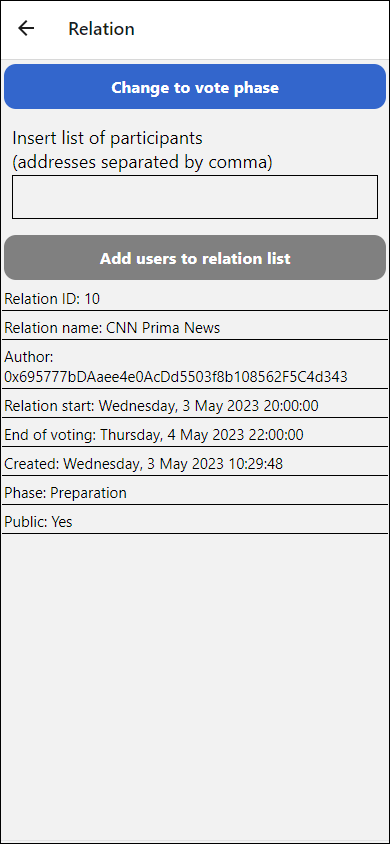
\includegraphics[width=.9\linewidth]{obrazky/konkretni_relace.png}
  \captionof{figure}{Zobrazení konkrétní relace \newline}
  \label{fig:konkretni_relace}
\end{minipage}
\end{figure}

\subsubsection*{mapping(uint=>Relation) relations}
K~uložení všech relací byla použita datová struktura \texttt{mapping}, která funguje jako asociativní pole nebo slovník v~jiných programovacích jazycích. Byla vybrána z~důvodu, protože poskytuje efektivní přístup k~datům při jejich velkém objemu pomocí mapování ID relace na strukturu relace. K~mappingu byla využita proměnná \texttt{numRelations}, která slouží jako čítač relací a uchovává jejich celkový počet.  
% k mappingu??
\subsection*{funkce addRelation}
Začněme tedy první funkcí, která samotnou relaci vytvoří. Moderátor při tvorbě relace zadává, zda je veřejná či soukromá, dále její název, její začátek a čas, do kdy lze zadávat v~relaci otázky. Čas vytvoření relace je stanoven podle hodnoty \texttt{block.timestamp}, ID je podle proměnné \texttt{numRelations}. Počáteční fází je vždy ta přípravná. Moderátor vytváří relace pomocí rozhraní aplikace znázorněného na obrázku \ref{fig:pridani_relace}. Funkce má speciální typ \texttt{payable}, který označuje, že se jedná o~transakci, která umožňuje poslat ether do smart kontraktu. Spuštění funkce je podmíněno tím, že má moderátor ověřenou identitu a že zaplatí požadovanou částkou za vytvoření relace. Výše požadované částky je pevně nastavena v~aplikaci. 
%ether - věta?
\subsection*{funkce addUsersToRelation}
Nyní se přesuneme k~funkci přidávající uživatele do soukromé relace. Vstupními podmínkami pro její úspěšný průběh jsou, že odesílatel transakce je sám autorem relace, dále, že relace je veřejná a nachází se v~přípravné fázi. Při splnění všech podmínek lze následně přidat uživatele jednotlivě nebo jako pole adres. Pole vytváří sama aplikace z~uživatelského vstupu, ve kterém jsou jednotlivé adresy oddělené čárkou. Obrázek \ref{fig:konkretni_relace} znázorňuje finální aplikaci, kde je zobrazen rámeček na vložení adres. Pod ním je tlačítko na odeslání transakce. Šedá barva symbolizuje jeho nefunkčnost a to z~důvodu, že se jedná o~veřejnou relaci, ve které nelze uživatele přidávat. Zároveň může mít šedou barvu i z~důvodu, že se relace nachází v~hlasovací fázi. V~opačném případě by bylo tlačítko zabarveno modře. Vložené adresy se zde mohou opakovat z~důvodu, že by mohla být transakce při kontrole stejných adres neúspěšná a bylo by zbytečně komplikované volat transakci znovu. Jelikož všechny ostatní funkce, které jsou zmíněné v~této sekci, mají kontrolu ověření adres, tak to není ani potřeba. 
%poslední souvětí?
\subsection*{funkce changeRelationPhase}
Zde se dostáváme k~poslední funkci přímo ovlivňující relace, a to změnu její fáze. Jak již bylo zmíněno na začátku této sekce, jde pouze o~jednorázovou záležitost. V~případě, že by se umožnilo moderátorovi měnit fáze opakovaně, mohl by nastat problém s~tím, že tímto způsobem bude moci omezovat účastníky, aby přidávali nové otázky a hlasovali, jelikož v~přípravné fázi lze pouze zvát účastníky. Jak je vidět na obrázku \ref{fig:konkretni_relace}, tlačítko je zabarveno modře, což znamená, že ho lze stisknout. Poté, co se fáze změní, tlačítko zešedne a moderátor již bude vědět, že změna fáze proběhla.
%první věta -množné a jednotné
\subsection{Otázky}
Nakonec se dostáváme k~samotným otázkám v~relacích a k~hlasování s~nimi spojeném. Datová struktura otázek je sama o~sobě poměrně strohá. Jak je vidět na úryvku kódu níže, tvoří ji pouze text, pole adres uchovávající hlasy dané otázky a její autor.
%její autor??? čí
\begin{verbatim}
struct Question {
    string text;
    address[] votes;
    address author;
}
\end{verbatim}  

\subsubsection*{mapping(uint=>Question) questions}
Jednotlivé dotazy jsou uloženy do mappingu \texttt{questions}, stejně jako tomu je u~relací. ID dotazů, které jsou uloženy v~relacích v~poli \texttt{questionKeys}, po vložení do mappingu \texttt{questions} vrátí konkrétní otázky, které lze posléze uživateli zobrazit. Není proto potřeba ani duplicitně ukládat jejich samotné ID.
%% celý mapping?
\subsection*{funkce addQuestion}
\texttt{AddQuestion} je funkcí zodpovědnou za vytvoření otázek a jejich přidávání do konkrétních relací. Její důležitou součástí je kontrola, zda uživatel již zadal otázku do relace. Ta má mít společně s~ověřením uživatele za cíl zamezení spamu otázek v~relacích. Uživatel se tak musí rozhodnout, jakou otázku chce položit a předem si ji dobře promyslet. V~případě soukromé relace probíhá kontrola odesílatele, jestli se nachází mezi pozvanými účastníky. Aplikace Voter zde ještě kontroluje délku zadané otázky, která má nanejvýš 200 znaků. Na obrázku \ref{fig:relace_otazky} je zobrazena konkrétní relace s~možností přidat otázku. Níže je vidět seznam otázek, který je seřazen podle počtu hlasů. 
% která má - může mít?
\subsection*{funkce voteForQuestion}
Druhou funkcí operující s~otázkami je \texttt{voteForQuestion}. Jejím úkolem je zařídit přidání hlasu (adresy odesílatele) ke konkrétní otázce. Hlasy zajišťují oblíbenost otázky, na jejich základě si může moderátor vybrat nejoblíbenější otázky publika. V~případě soukromé relace zde probíhá stejná kontrola, jako při vytváření otázek. Navíc se zde kontroluje, zda již uživatel hlasoval pro danou otázku a zamezilo se tak duplicitnímu hlasování. Zobrazení hlasů a možnost hlasování lze vidět na obrázku \ref{fig:konkretni_otazka}.
% na jejich - na jejichž
% publika - z publika?
\begin{figure}
\centering
\begin{minipage}{.5\textwidth}
  \centering
  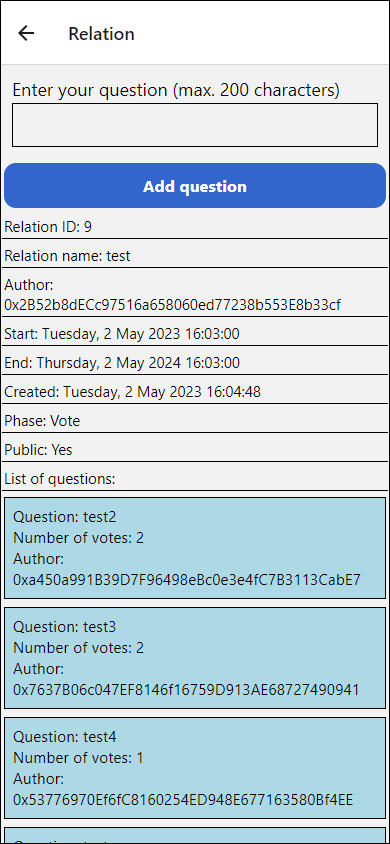
\includegraphics[width=.9\linewidth]{obrazky/relace_s_otazkami.png}
  \captionof{figure}{Relace s~otázkami}
  \label{fig:relace_otazky}
\end{minipage}%
\begin{minipage}{.5\textwidth}
  \centering
  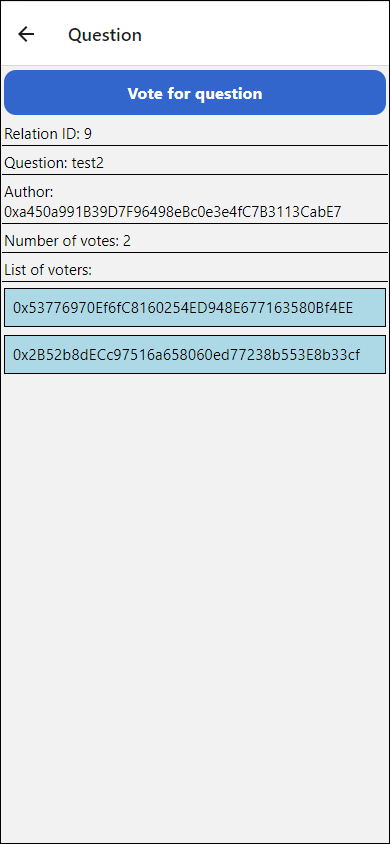
\includegraphics[width=.9\linewidth]{obrazky/konkretni_otazka.png}
  \captionof{figure}{Konkrétní otázka}
  \label{fig:konkretni_otazka}
\end{minipage}
\end{figure}

\chapter{Evaluace a zhodnocení}
\label{chapter:7}
Procesem testování by měl správně procházet vývoj všech aplikací. Proto zde představím postupy, které byly uplatněny při testování výsledných aplikací a smart kontraktů. Testy probíhaly již od prvního návrhu smart kontraktu a byly postupně upravovány podle potřeby. V~druhé části kapitoly si probereme nedostatky a možné budoucí rozšíření aplikace a zhodnotíme výsledek práce. 

\section{Testování}
\subsection*{Unit testy}
První způsob testování se zaměřoval na funkčnost smart kontraktů \texttt{Queans} a \texttt{identity\-Registry}. Testy probíhaly na základě změn smart kontraktu \texttt{Queans}, které byly potřeba provést po jeho rozšíření, a měly za úkol kontrolovat, že všechny funkce se chovají správným způsobem. Jednalo se hlavně o~kontrolu stavů, ve kterých by funkce neměla projít, jelikož nesplnila některou z~podmínek pro její korektní průchod. K~tomu byly využity unit testy s~použitím platformy Truffle Suite. Unit testy jsou rozděleny do 2 částí, první se zaměřuje na smart kontrakt \texttt{identityRegistry}, jehož správné chování je nezbytné pro fungování smart kontraktu \texttt{Queans}, který se nachází v~druhé části testů. Testují se všechny funkce, které mohou měnit stav blockchainu. Nejčastěji odhalené chyby byly zpravidla špatně zvolené relační operátory nebo chybná práce s~datovými strukturami.
% rozšíření - změně? změnách?
\subsection*{Konzole a pomocné nástroje}
Druhým způsobem testování, které bylo použito během tvorby aplikací je zpětná vazba zejména z~chybových výpisů v~konzoli, statusu transakcí u~nástroje Etherscan či Truffle nebo peněženky Metamask. Konzolové výpisy společně s~nástrojem Etherscan dokázaly odhalit, v~jaké části funkce nastala chyba, která byla omylem zanesena do aplikace. Peněženka Metamask se prakticky vždy, kdy má dojít k~neúspěšné blockchainové transakci, dotazuje, zda má být konkrétní transakce provedena. Tudíž ještě před utracením prostředků dochází k~varování uživatele. I~přes úspěšné unit testy docházelo v~aplikaci k~chybnému zapsání kódu pro volání funkcí smart kontraktu, kde nebyly zpravidla rozlišeny metody \texttt{call} od \texttt{send} či byly zcela opomenuty. Chybové konzolové výpisy odhalovaly hlavně špatné použití komponent frameworku React Native.  
% TODO
% byly zcela opomenuty - čárka před či?
%ˇtvorby aplikací - *čárka* je zpětnýá vazba
% call a send - při komunikaci se smart kontraktem?
\section{Diskuze}
Nejprve bych zmínil, že během vývoje došlo k~odchylce od zadání práce, kde namísto mobilní aplikace byly implementovány aplikace webové, k~čemuž jsem se uchýlil ze dvou důvodů. Prvním bylo uvědomění si, že proces pokládání otázek a hlasování by měl být co možná nejsnažší, aby neodradil uživatele. K~tomu mi přispěla analýza současných aplikací ze sekce \ref{analyza}, kde jsem zjistil, že všechny existující aplikace jsou webové, protože si uživatel nemusí stahovat žádnou aplikaci a rychleji se může zapojit. Druhým důvodem, který vedl k~tomuto rozhodnutí, se stal fakt, že peněženka Metamask vykazovala nekonzistentní chování při připojení se k~aplikaci, což by vedlo k~špatné uživatelské zkušenosti. Na obrázku \ref{fig:chyby} je vyobrazen screenshot konzole a emulátoru mobilního telefonu, kde se aplikace připojuje k~peněžence, ale nedojde k~samotnému připojení. Při pokusu o~opětovné připojení se vyskytují chybová hlášení \texttt{Keys are not exchanged} a následně \texttt{Wrong id}. Podle vlastního testování se toto chování ještě zhoršilo po importu knihovny \texttt{web3}. Přestože jsem se několikrát po delší čekací době úspěšně připojil do peněženky, spojení s~peněženkou bylo záhy přerušeno. Mimo Metamask SDK jsem vyzkoušel i službu WalletConnect, která bohužel ve verzi 1.x.x pro React Native nefungovala a již není aktualizovaná a verze 2.x.x pro React Native ještě není dokončena, kde termín dokončení je stanoven na konec června letošního roku 2023. V~případě, že bude jedna z~těchto možností funkční, není problém dokončit práci podle stanoveného zadání. Úprava by spočívala pouze v~úpravě funkce \texttt{load} ve zdrojovém kódu decentralizovaných aplikací, kde by se podle podmínky níže byla aplikace schopná napojit přímo na aplikaci mobilní peněženky Metamask. Všechny ostatní funkce by nepotřebovaly žádnou dodatečnou změnu a měly by být plně funkční.
% rychleji se může zapojit - do relace - komunikace, ...
% připojení se k aplikaci? se??
% by nepotřebovaly - nepotřebují
\begin{verbatim}
if (Platform.OS === 'web') {
    //aktuální způsob připojení
} else if (Platform.OS === 'ios' || Platform.OS === 'android') {
    //nové připojení na mobilní aplikace peněženky Metamask
}
\end{verbatim}

\subsection{Nedostatky současných aplikací}
\label{nedostatky}
Současný stav aplikací provází několik nedostatků, které by měly být opraveny. První nedostatek spočívá v~samotném designu aplikací. Uživatelské prostředí nevypadá dvakrát přívětivě a rozhodně by stálo ho upravit tak, aby bylo pro uživatele vlídnější. K~dalšímu nedostatku bych zařadil způsob zadávání datumů a času při tvorbě relace. Uživatel se může snadno přepsat a udělat tak chybu, která již nepůjde opravit. Nicméně se mi nepodařilo nalézt vhodnou knihovnu, která by byla kompatibilní pro mobilní a webové aplikace zároveň a nabízela jednoduchou volbu datumu a času pomocí jednoho vstupu. Jako poslední nedostatek je nutnost manuálního přepnutí fáze relace, aby bylo uživatelům umožněno pokládání otázek a hlasování. Moderátorovi se může snadno stát, že zapomene fázi změnit a do relace se následně nedostanou žádné otázky.
%jednoho - jednotného?
\subsection{Budoucí rozšíření aplikací}
V~případě, že by aplikace měly dojít do stavu, kdy by mohly být použity širší veřejností, je třeba je ještě rozšířit a opravit nedostatky zmíněné v~předchozí sekci \ref{nedostatky}. Přestože aplikace fungují, jak mají, pro širší adopci je zejména důležitý jejich vzhled, který by bylo nutné přepracovat. Dále by bylo dobré přidat filtrování relací podle toho, zda se jedná o~nadcházející, probíhající či ukončené relace. Pro zvýšení atraktivnosti je dalším krokem zavedení motivačního modelu, který je popsán v~sekci \ref{protokol}. Ten by motivoval uživatele k~větší interakci s~vidinou finanční nebo jiné odměny, která by byla důležitá zejména pro rozšíření aplikací mezi více uživatelů a tím by mohly získat větší popularitu. Další možností rozvoje je okamžitá aktualizace dat po provedení úspěšné blockchainové transakce, která funguje aktuálně při přidání nové relace, nicméně např. při přidání hlasů se musí uživatel vrátit na přehled relací a zpět na konkrétní otázku, aby viděl nově přidaný hlas.

\begin{figure}
\centering
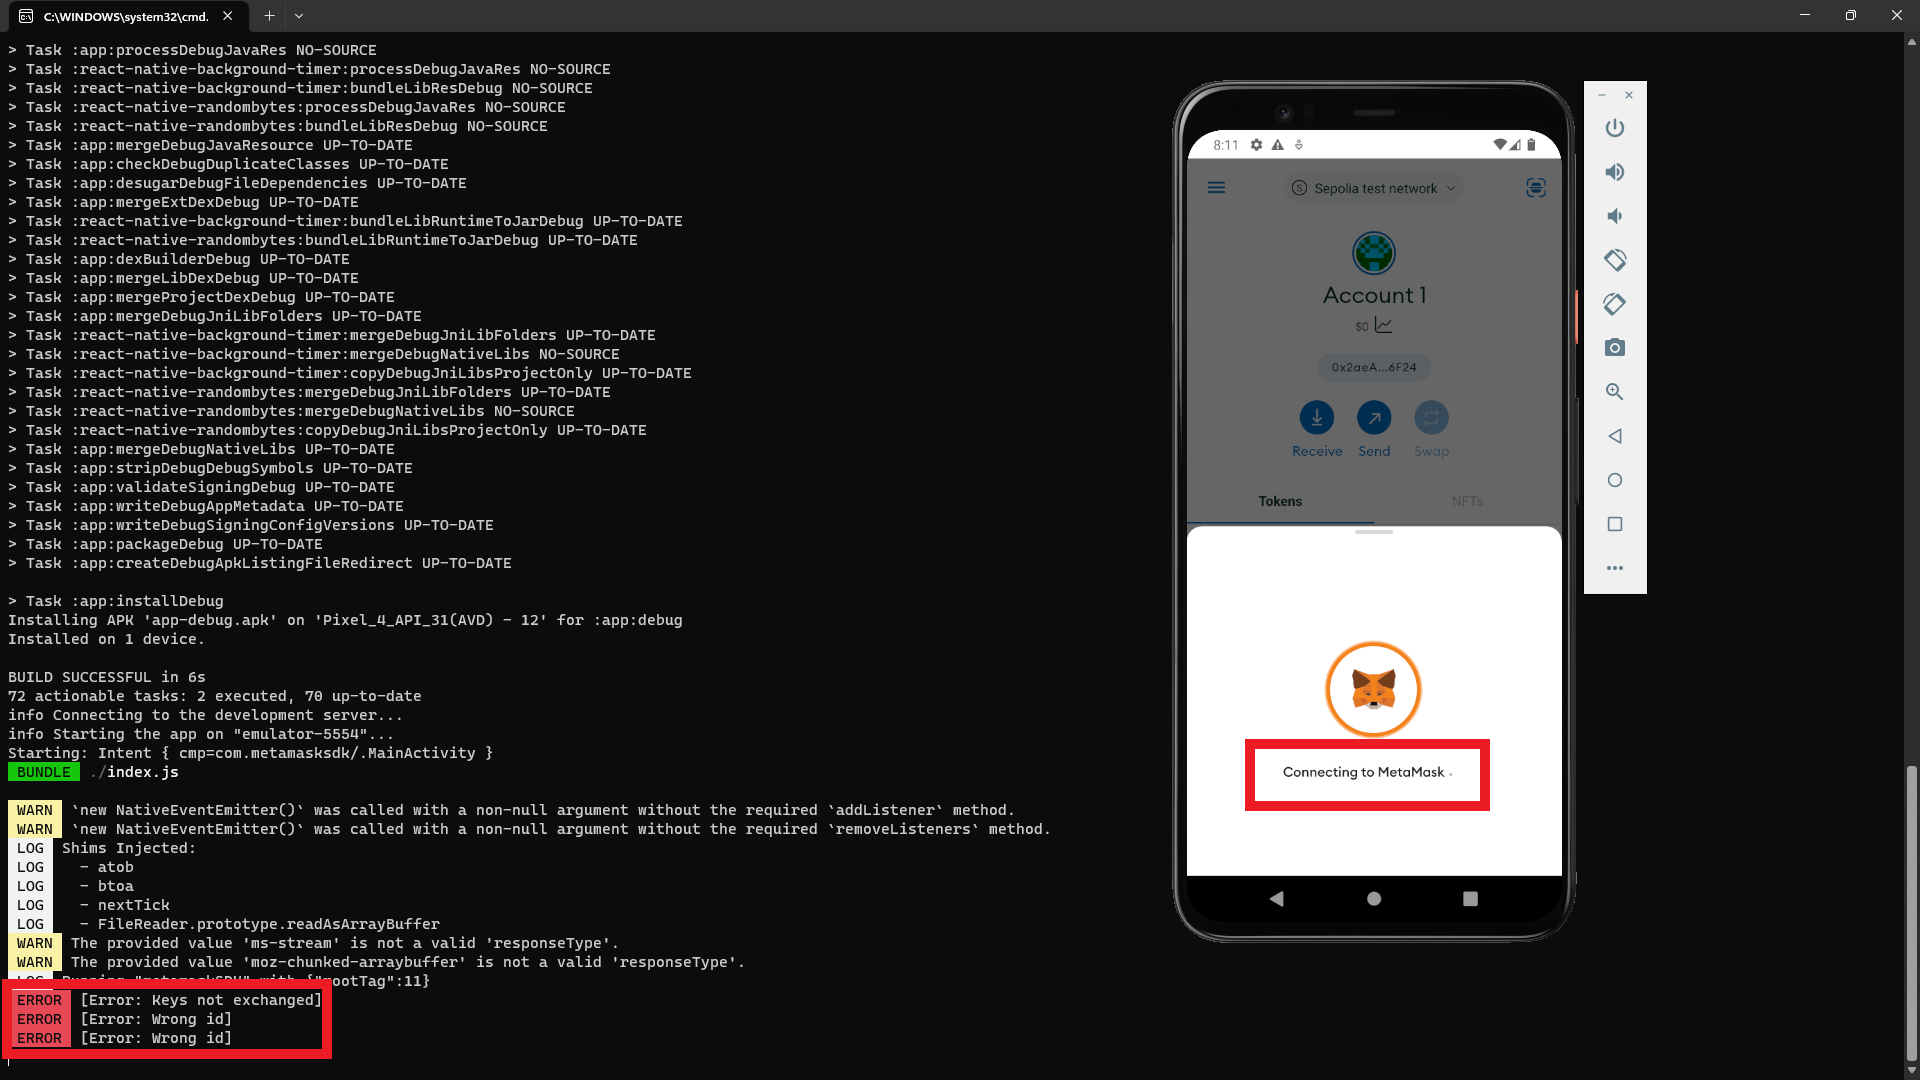
\includegraphics[width=\linewidth]{obrazky/dukaz.png}
\caption{Chyby}
\label{fig:chyby}
\end{figure}

\section{Bezpečnostní analýza}
V~této sekci se podíváme na situace, které by mohly nastat v~případě zneužití práv, která mají jednotliví aktéři aplikací.  
\subsection{Nevhodné chování poskytovatele identit}
\label{poskytovatel}
Nejprve se podíváme na možné problémy u~poskytovatele identity. Co by se stalo, kdyby se choval tak, že odmítne ověřit uživatele po předložení identity? Uživatel bude mít možnost si vybrat, ke kterému poskytovateli identity půjde. V~případě, že by ho někdo nechtěl ověřit, není problém vyhledat jiného poskytovatele a ověřit se u~něho. 

Další problém by mohl nastat ve chvíli, kdy poskytovatel identity bude přidávat ověřené uživatele s~úmyslem poškodit celou aplikaci nebo relaci. Mohl by tak vytvořit nespočet uživatelů, kteří by mohli zahlcovat relace nevhodnými dotazy či neustále vytvářet nové relace, které by znepřehledňovali aplikace. Na tyto problémy navážeme v~sekci \ref{nevhodne}. 

Je přidání centralizovaného poskytovatele identity snížením decentralizace všech aplikací? Dalo by se říci, že ano, ale jen trochu. Aplikace pro správu identit je jen jednou z~částí Q\&A relací.  Centralizace nebude tak velká, protože poskytovatelů identity bude celá řada. Mimo to známe jejich identitu a v~případě jejich nekorektního chování by bylo možné s~nimi zúčtovat. 
% s nimi zúčtovat
\subsection{Nevhodné chování uživatelů}
\label{nevhodne}
Nyní se dostáváme k~uživatelům a přesuneme se na tvorbu nevhodných otázek v~relaci, což by mohlo částečně souviset i se spamem. Prvním prvkem, který částečně limituje množství těchto zpráv, je maximální počet otázek, který mohou uživatelé položit, s~aktuální hodnotou 1. Díky tomu, že aplikace nikomu neumožňuje cenzurovat žádné otázky, se může stát, že se v~relacích nevhodné dotazy objeví. V~případě, že by nastal problém s~poskytovatelem identit popisovaný v~předchozí sekci \ref{poskytovatel}, který by ověřil účty bez poskytnutí identity, se zde nachází další prvek zamezující nevhodnému chování v~podobě ceny za položení otázky (aktuálně je cena na nízké úrovni, aby se dalo aplikaci otestovat, v~případě nasazení aplikace by se ale zavedla cena, která by nebyla tak nízká). Útočník by následně musel vynaložit určité množství prostředků, aby vytvořil více otázek. To však nemění nic na tom, že pokud pro tyto otázky nebudou ostatní uživatelé hlasovat, tak skončí na nižších pozicích a moderátor se o~ně nebude zajímat. 

Dalším typem útoku by mohlo být nadměrné vytváření relací. Proti tomuto problému by měla zasáhnout opět cena za vytvoření relace. Další možností je možnost ověření uživatelů, že konkrétní relace vznikla z~adresy, kterou propaguje moderátor či organizátor relace. Ti by uživatelům měli také poskytnout ID relace, aby ji jednoduše vyhledali.
%další možností je možnost
\section{Zhodnocení aplikací}
Mezi výhody aplikací bych zařadil jejich jednoduché rozhraní, které není složité na pochopení. Dále, že se jedná o~funkční projekt, který úspěšně demonstruje, jak by aplikace mohla vypadat a být použita. Třetí výhodou je fakt, že aplikace byly nakonec vytvořeny jako webové a nabízí tak snažší použití pro uživatele. Navíc jsou dostupné i na počítači, což není rozhodně na škodu. 

Jako nevýhody lze zařadit již zmíněné nedostatky, které se objevily, zejména nutnost manuálního přepnutí fáze relace, na kterou si musí aktuálně moderátor dávat pozor. S~tím je následně spojena i nemožnost pokládat otázky do relace a hlasovat. Nevýhodou také může být nepřehlednost zobrazení relací při jejich vyšším počtu, kde ale funguje možnost filtrování podle ID relace, které by měl uživatel obdržet od moderátora.
% zde uvést dlouhé načtení při velkém monžství relací a otázek?
\chapter{Závěr}
Cílem práce bylo vytvořit decentralizovanou mobilní aplikaci poskytující Q\&A sekci s~využitím blockchainu. Mezi hlavní přednosti aplikací se řadí odolnost vůči cenzuře, kterou nabízí propojení s~blockchainem a zamezení spamu, čehož bylo docíleno pomocí propojení se systémem pro správu identit poskytnutým od doktora Homoliaka.
% TODO_HM 
% + 2. věta doplnit Výslednou aplikace jsem rozdělil do 3 separátních, které dávají větší smysl?

Před začátkem práce bylo zapotřebí prostudovat problematiku blockchainu, smart kontraktů a decentralizovaných aplikací, která mi pomohla objasnit, jak jsou na sobě zmíněné pojmy závislé. Následně jsem studoval programovací prostředí vhodné pro mobilní aplikace, které mi pomohlo k~rozhodnutí, jak aplikace tvořit. Na konci teoretické části jsou popsány použité technologie, které byly nezbytnou součástí při tvorbě výsledných aplikací.

Na začátku praktické části popisuji již existující centralizované aplikace a zhodnocuji výhody a nevýhody jednotlivých řešení. Poté se již přesouvám k~samotnému návrhu aplikace a protokolu, podle kterého následně proběhla implementace aplikací. V~úplném závěru práce je popsán způsob testování společně s~nedostatky a možnými rozšířeními aplikace.

Výsledek práce byl splněn s~rozdílem, že místo mobilní aplikace byly vytvořeny aplikace webové. K~tomu došlo ze dvou důvodů. Prvním je, aby se uživatelé mohli rychleji a snáze zapojit do relace. Druhý důvod je aktuální nekonzistentní chování kryptoměnové peněženky Metamask. Nakonec bych změnu označil za pozitivní a výsledné aplikace díky ní nabízejí lepší vlastnosti. 

Do budoucna bych rád otestoval aplikace v~reálných podmínkách a zkusil je nabídnout organizátorům přednášek, od kterých bych následně dostal cennou zpětnou vazbu. Jako rozšíření by bylo do aplikace vhodné implementovat filtrování relací podle různých klíčů, aby bylo uživatelům usnadněno vyhledávání relací nejenom podle jejich ID a zobrazení relací by se následně stalo přehlednějším. 

Bakalářská práce byla mým nejrozsáhlejším samostatným projektem a naučila mne být více samostatný při řešení různých problémů. Také jsem si osahal postupy tvorby mobilních aplikací, ve kterých bych v~budoucnu rád pokračoval. Největším přínosem pro mne však bylo hlubší pochopení problematiky blockchainu, protože v~něm vidím veliký potenciál a osobně mě tato oblast zajímá.
% TODO_HM 
% psát v 1. osobě? já já já?
% názvy obrázků
% předělat poslední odstavec, takhle se mi to nelíbí

% doplnit v rozšíření - cache? dlouhé načítání při velkém množství dat? nedostatek?